\documentclass{umthesis}          % for Ph.D. dissertation or proposal

\usepackage{graphicx}
\usepackage{epsfig}
\usepackage{amssymb}
\usepackage{amsfonts}
\usepackage{verbatim}
\usepackage{moreverb}
\usepackage{cancel}
\usepackage{fancyhdr}
\usepackage{algorithmic}
\usepackage[algosection,lined,linesnumbered,ruled]{algorithm2e}
%\usepackage[algochapter,lined,linesnumbered,ruled]{algorithm2e}
\usepackage{epstopdf}
\usepackage{amssymb,amsfonts,amsmath,amsthm}
\usepackage{subfigure}

\usepackage{rotating}
\usepackage{framed}
\usepackage{xcolor}
\usepackage{soul}
\usepackage{fancyhdr}
\usepackage{enumerate}
\usepackage{cancel}
\usepackage{endnotes}
\usepackage{datetime}
\usepackage{hyperref}  %does not compile when using this line


\newtheorem{theorem}{Theorem}[chapter]
%\setcounter{theorem}{0}
\newtheorem{claim}[theorem]{Claim}
\newtheorem{conjecture}[theorem]{Conjecture}
\newtheorem{corollary}[theorem]{Corollary}
\newtheorem{fact}[theorem]{Fact}
\newtheorem{lemma}[theorem]{Lemma}
\newtheorem{meta-proposition}[theorem]{Meta-Proposition}
\newtheorem{note}[theorem]{Note}
\newtheorem{observation}[theorem]{Observation}
\newtheorem{proposition}[theorem]{Proposition}
\newtheorem{proviso}[theorem]{Proviso}         
\newtheorem{question}[theorem]{Question}         
\newtheorem{remark}[theorem]{Remark}         
\newtheorem{define}{Definition}     


%%%%%%%%%%%%%%%  ROLLBACK MACROS  %%%%%%%%%%%%%%%%%%%%%%%%%%%%%%%%%%%%%%%%
\newcommand{\minv}{$\overrightarrow{min}$ }
\newcommand{\minvi}{$\overrightarrow{min}_i$ }
\newcommand{\minvis}{$\overrightarrow{min}_i$}
\newcommand{\minvj}{$\overrightarrow{min}_j$ }
\newcommand{\minvjs}{$\overrightarrow{min}_j$}
\newcommand{\minvv}{$\overrightarrow{min}_v$ }
\newcommand{\minvvs}{$\overrightarrow{min}_v$}
\newcommand{\dmatrix}{$dmatrix$ }
\newcommand{\dmatrixs}{$dmatrix$}
\newcommand{\dmatrixi}{$dmatrix_i$ }
\newcommand{\dmatrixis}{$dmatrix_i$} 
\newcommand{\dmatrixj}{$dmatrix_j$ }
\newcommand{\dmatrixjs}{$dmatrix_j$} 
\newcommand{\dmatrixv}{$dmatrix_v$ }
\newcommand{\dmatrixvs}{$dmatrix_v$} 
\newcommand{\dv}{{DV$^+$ }}
\newcommand{\Bad}{{$\overline{V}$ }}
\newcommand{\Bads}{{$\overline{V}$}}
\newcommand{\bad}{{$\overline{v}$ }}
\newcommand{\bads}{{$\overline{v}$}}
\newcommand{\alg}{{DV$^+$ }}
%\newcommand{\infinity}{{count-to-$\infty$ }}
\newcommand{\infinity}{{count-to-infinity }}


\newcommand{\second}{\textsc{2nd-Best} }
\newcommand{\seconds}{\textsc{2nd-Best}}  
\newcommand{\purge}{{\textsc{Purge} }}
\newcommand{\purges}{{\textsc{Purge}}}
\newcommand{\cpr}{\textsc{CPR} }
\newcommand{\cprs}{\textsc{CPR}}
%\newcommand{\second}{{{\tt 2}$^{{\tt nd}}$ {\tt best} }}
%\newcommand{\seconds}{{{\tt 2}$^{{\tt nd}}$ {\tt best}}}
%\newcommand{\purge}{{{\tt purge} }}
%\newcommand{\purges}{{{\tt purge}}}
%\newcommand{\cpr}{{\tt cpr} }
%\newcommand{\cprs}{{\tt cpr}}

\newcommand{\badvector}{$\overrightarrow{bad}$ }
\newcommand{\badvectors}{$\overrightarrow{bad}$}
\newcommand{\oldvector}{$\overrightarrow{old}$ }
\newcommand{\oldvectors}{$\overrightarrow{old}$}
\newcommand{\finalvector}{{$v_{final}$ }}
\newcommand{\illigit}{{illegitimate path} }
\newcommand{\illigits}{{illegitimate paths} }
\newcommand{\lcd}{$\Delta_{lc}$ }
\newcommand{\lcds}{$\Delta_{lc}$s }

\newcommand{\er}{Erd\"{o}s-R\'enyi }
\newcommand{\ers}{Erd\"{o}s-R\'enyi} 

\newcommand{\etal}{el al.}



%%%%%%%%%%%%%%%  PMU PLACEMENT MACROS  %%%%%%%%%%%%%%%%%%%%%%%%%%%%%%%%%%%%%%%%
\newcommand{\sat}{{\textsc{P3SAT} }}
\newcommand{\sats}{{\textsc{P3SAT}}}
\newcommand{\full}{{\textsc{FullObserve} }}
\newcommand{\fulls}{{\textsc{FullObserve}}}
\newcommand{\maxinc}{{\textsc{MaxObserve} }}
\newcommand{\maxincs}{{\textsc{MaxObserve}}}
\newcommand{\xval}{{\textsc{FullObserve-XV} }}
\newcommand{\xvals}{{\textsc{FullObserve-XV}}}
\newcommand{\xvalpart}{{\textsc{MaxObserve-XV} }}
\newcommand{\xvalparts}{{\textsc{MaxObserve-XV}}}


%%%%%%%%%%%%%%%  MULTICAST RECOVERY MACROS  %%%%%%%%%%%%%%%%%%%%%%%%%%%%%%%%%%%%%%%%


\newcommand{\cnt}{{\tt count} }
\newcommand{\cnts}{{\tt count}}

\newcommand{\mf}{\textsc{Min-Flows} }
\newcommand{\mfs}{\textsc{Min-Flows}}
\newcommand{\mds}{\textsc{Min-Sinks}}
\newcommand{\md}{\textsc{Min-Sinks} }
\newcommand{\mdj}{\textsc{Max-Disjoint} }
\newcommand{\mdjs}{\textsc{Max-Disjoint}}

%\newcommand{\mdr}{\textsc{Monitor-Detect-Recover} }
%\newcommand{\mdrs}{\textsc{Monitor-Detect-Recover}}
\newcommand{\mdr}{\textsc{Appleseed} }
\newcommand{\mdrs}{\textsc{Appleseed}}

\newcommand{\mc}{\textsc{Multicast Recycling} }
\newcommand{\mcs}{\textsc{Multicast Recycling}}
\newcommand{\mcn}{Multicast Recycling }
\newcommand{\mco}{\textsc{1Multicast Recycling} }
\newcommand{\mcos}{\textsc{1Multicast Recycling}}

\newcommand{\pre}{\textsc{Proactive} }
\newcommand{\pres}{\textsc{Proactive}}
\newcommand{\preroot}{\textsc{Kotani} }
\newcommand{\preroots}{\textsc{Kotani}}


\newcommand{\post}{\textsc{Reactive} }
\newcommand{\posts}{\textsc{Reactive}}

\newcommand{\mdst}{{\tt 111.111.111.111} }
\newcommand{\mdsts}{{\tt 111.111.111.111}}

\newcommand{\steiner}{\textsc{Bunchy} }
\newcommand{\steiners}{\textsc{Bunchy}}
\newcommand{\steinern}{Bunchy }
\newcommand{\arbor}{\textsc{Steiner-Arborescence} }
\newcommand{\arbors}{\textsc{Steiner-Arborescence}}

\newcommand{\merge}{\textsc{Merger} }
\newcommand{\merges}{\textsc{Merger}}
\newcommand{\mergen}{Merger }

\newcommand{\base}{\textsc{Basic} }
\newcommand{\bases}{\textsc{Basic}}
\newcommand{\basen}{Basic }

\newcommand{\lb}{\textsc{LB} }
\newcommand{\lbs}{\textsc{LB}}

\newcommand{\pcnt}{\textsc{Pcount} }
\newcommand{\pcnts}{\textsc{Pcount}}




%%%%%%%%%%%%%%%  SELF-NOTE AND TODO  MACROS  %%%%%%%%%%%%%%%%%%%%%%%%%%%%%%%%%%%%%%%%
\newcommand{\xx}[1] {\textcolor{purple}{ {\bf \underline{Question}: #1 ????}}} %question
\newcommand{\xxn}[1] {\textcolor{purple}{#1}}  % question

\newcommand{\xxx}[1] {\textcolor{orange}{\textit{\underline{Self Note}: #1}}} % Self-Note
\newcommand{\xxxe}[1] {\endnote{ \textcolor{orange}{#1}}} % Self-Note
\newcommand{\xxxn}[1] {\textcolor{orange}{#1}} % Self-Note

\newcommand{\todo}[1] {\textcolor{cyan}{\textit{{\bf TODO}  #1}}} % Todo notes
\newcommand{\xxxx}[1] {\textcolor{cyan}{\textit{{\bf TODO}  #1}}} % Todo notes
\newcommand{\xxxxe}[1] {\endnote{ \textcolor{cyan}{\textit{{\bf TODO}  #1}}}} % Todo notes
\newcommand{\xxxxn}[1] {\textcolor{cyan}{#1}} %  % Todo notes

\newcommand{\yy}[1] {\endnote{ {\textcolor{gray}{\underline{Comment}: {\it #1}}}} }  %maybe text
\newcommand{\yyn}[1] {\textcolor{gray}{#1}} %maybe text

%\newcommand{\un}[1]{%
%    \ifmmode \@@underline{#1} \else %
%             $\@@underline{\hbox{#1}}$\fi}

\begin{document}

\title{Making Networks Robust to Component Failure}
\author{Daniel P. Gyllstrom}
\date{(Compiled on \mmddyyyydate\today\ at \currenttime)}
%\date{January 2013} % The date you'll actually graduate -- must be
                     % February, May, or September
\copyrightyear{2013}
\bachelors{B.Sc.}{Trinity College}
\masters{M.Sc.}{University of Massachusetts Amherst} 
\committeechair{Jim Kurose}
\firstreader{Prashant Shenoy}
\secondreader{Deepak Ganesan}
\thirdreader{Lixin Gao}  
\departmentchair{Lori Clarke}
\departmentname{Computer Science}

\degree{Doctor of Philosophy}{Ph.D.}

%%
%% These lines produce the title, copyright, and signature pages.
%% They are Mandatory; except that you could leave out the copyright page
%% if you were preparing an M.S. thesis instead of a PhD dissertation.
\frontmatter
%\maketitle
%\copyrightpage     %% not required for an M.S. thesis
%\signaturepage

%%
%% Dedication is optional -- but this is how you create it
%\begin{dedication}              % Dedication page
%  \begin{center}
%    \emph{For myself.}
%  \end{center}
%\end{dedication}


%\chapter{Acknowledgments}             % Acknowledgements page
%  Thanks to me. 


%\begin{abstract}

Communication network components -- routers, links connecting routers, and sensors -- inevitably fail, causing service outages and a potentially unusable network. 
Recovering quickly from these failures is vital to both reducing short-term disruption and increasing long-term network survivability. 
In this thesis, we consider instances of component failure in the Internet and in networked cyber-physical systems, such as the communication network used by the modern electric power grid 
(termed the \emph{smart grid}). 
We design algorithms that make these networks more robust to component failure.
This thesis divides into three parts: (a) recovery from malicious or misconfigured nodes injecting false information into a distributed system (e.g., the Internet), (b) placing smart grid sensors to provide measurement error detection, and 
(c) fast recovery from link failures in a smart grid communication network. 



First, we consider the problem of malicious or misconfigured nodes that inject and spread incorrect state throughout a distributed system.
Such false state can degrade the performance of a distributed system or render it unusable. For example, in the case of network routing algorithms, false state corresponding
to a node incorrectly declaring a cost of $0$ to all destinations (maliciously or due to misconfiguration) can quickly spread through the network. This causes other nodes to (incorrectly) 
route via the misconfigured node, resulting in suboptimal routing and network congestion. We propose three algorithms for efficient recovery in such scenarios and evaluate their efficacy.


The last two parts of this thesis consider robustness in the context of the electric power grid. 
We study a type of sensor, a Phasor Measurement Unit (PMU), currently being deployed in electric power grids worldwide. 
PMUs provide voltage and current measurements at a sampling rate orders of magnitude higher than the status quo.  As a result, PMUs can 
both drastically improve existing power grid operations and enable an entirely new set of applications, such as the reliable integration of renewable energy resources. 
However, PMU applications require \emph{correct} (addressed in thesis part 2) and \emph{timely} (covered in thesis part 3) PMU data. 
Without these guarantees, smart grid operators and applications may make incorrect decisions and take corresponding (incorrect) actions. 

The second part of this thesis addresses PMU measurement errors, which have been observed in practice. 
We formulate a set of PMU placement problems that aim to satisfy two constraints: place PMUs ``near'' each other to allow
for measurement error detection and use the minimal number of PMUs to infer the state of the maximum number of system buses and transmission lines. 
For each PMU placement problem, we prove it is NP-Complete, propose a simple greedy approximation algorithm, and evaluate our greedy solutions.


%This is a three-part problem: (a) link failure detection, (b) algorithms for pre-computing backup multicast trees, and (c) fast installation of these backup trees.
In the last section of this thesis, we design algorithms for fast recovery from link failures in a smart grid communication network. 
We propose, design, and evaluate solutions to all three aspects of link failure recovery: (a) link failure detection, (b) algorithms for pre-computing backup multicast trees, and
(c) fast backup tree installation. 

To address (a), we design link-failure detection and reporting mechanisms that use OpenFlow to detect link failures when and where they occur \emph{inside} the network.
OpenFlow is an open source framework that cleanly separates the control and data planes for use in network management and control.
For part (b), we formulate a new problem, \mcs, that pre-computes backup multicast trees that aim to minimize control plane signinaling overhead. We prove \mc 
is at least NP-hard and present a corresponding approximation algorithm.
Lastly, two control plane algorithms are proposed that signal data plane switches to install pre-computed backup trees. 
An optimized version of each installation algorithm is designed that finds a near minimum set of forwarding rules 
by sharing forwarding rules across multicast groups. This optimization
%by using OpenFlow to dynamically write (and delete) identifiers in packet headers to allow forwarding rules to be shared across multicast groups. This optimization
reduces backup tree install time and control state.  
We implement these algorithms using the POX open-source OpenFlow controller and evaluate them using the Mininet emulator. 
		

%for fast installation of backup trees that both use OpenFlow to signal switches to install backup trees. 
%An optimization applied to each installation algorithm is designed to speed backup tree installation and reduce the amount of pre-installed control state.
%by identifying common forwarding behavior across multicast groups and using OpenFlow to dynamically write identifiers in packet headers to allow forwarding rules to be shared across multicast groups.
%consolidating forwarding rules in cases where multiple multicast trees have the same forwarding behavior. 

\end{abstract}





%%
%% Table of contents is mandatory, lists of tables and figures are 
%% mandatory if you have any tables or figures; must be in this order.
%\tableofcontents                % Table of contents
%\listoftables                   % List of Tables
%\listoffigures                  % List of Figures




%%%%%%%%%%%%%%%%%%%%%%%%%%%%%%%%%%%%%%%%%%%%%%%%%%%%%%%%%%%%%%%%%%%%%%%%%
%% Time for the body of the dissertation
\mainmatter   %% <-- This line is mandatory

%%
%% If you want an introduction, which is not a numbered chapter, insert
%% the following two lines.  This is OPTIONAL:

%\unnumberedchapter{Introduction}


\chapter{Recovery from Link Failures in a Smart Grid Communication Network}
\label{ch:reliable-mcast}

\section{Introduction}
\label{sec:intro-pmu}

\begin{framed}
\xxxxn{TODO Notes from Proposal Defense:}
\begin{itemize}
        \item \xxxxn{Lixin: Approximation bounds using modularity/sub-modular functions.  } 
	
	\item \xxxxn{Lixin: mention in future work (may already do this) that with special topologies you may be able to find more efficient algorithms for PMU placement.}

	\item \xxxxn{State Aazami et al show that the approximation for greedy algorithm is $\Theta(n)$, under the assumption that all nodes are zero-injection.  }
\end{itemize}
\end{framed}
               


This chapter considers placing electric power grid sensors, called phasor measurement units (PMUs), to enable measurement error detection.
%\xx{move paragraph to Smart Grid Overview Chapterr}
Significant investments have been made to deploy PMUs on electric power grids worldwide. PMUs provide \emph{synchronized} voltage and current measurements at a sampling rate orders 
of magnitude higher than the status quo: $10$ to $60$ samples per second rather than one sample every $1$ to $4$ seconds.  This allows system operators to directly measure the state of the electric power grid in real-time, rather than 
relying on imprecise state estimation. Consequently, PMUs have the potential to enable
an entirely new set of applications for the power grid:  protection and control during abnormal conditions, real-time distributed control, postmortem analysis of system faults,
advanced state estimators for system monitoring, and the reliable integration of renewable energy resources \cite{Naspi10}.

%\xx{move paragraph to Smart Grid Overview Chapter}
An electric power system consists of a set of buses  -- electric substations, power generation centers, or aggregation points of electrical loads -- and transmission lines connecting those buses.
The state of a power system is defined by the voltage phasor -- the magnitude and phase angle of electrical sine waves -- of all system buses and the current phasor of all transmission lines.
PMUs placed on buses provide real-time measurements of these system variables.
However, because PMUs are expensive, they cannot be deployed on all system buses \cite{Baldwin93}\cite{LaRee10}. Fortunately, the voltage phasor at a system bus can, at times, 
be determined (termed {\it observed} in this thesis) even when a PMU is not placed at that bus, by applying Ohm's and Kirchhoff's laws
on the measurements taken by a PMU placed at some nearby system bus \cite{Baldwin93}\cite{Brueni05}. Specifically, with correct placement of enough PMUs at a subset of system buses, the entire system state can be determined. 

In this chapter, we study two sets of PMU placement problems.  The first problem set consists of \full and \maxincs, and considers maximizing the observability of the network via PMU placement. \full considers the minimum number of PMUs needed 
to observe all system buses, while \maxinc considers the maximum number of buses that can be observed with a given number of PMUs. 
A bus is said to be {\em observed} if there is a PMU placed at it or if
its voltage phasor can be calculated using Ohm's or Kirchhoff's Law.  Although \full is well studied \cite{Baldwin93,Brueni05,Haynes02,Mili90,Xu04}, existing work considers only networks consisting solely of zero-injection buses, 
an unrealistic assumption in practice,
while we generalize the problem formulation to include mixtures of zero and  non-zero-injection buses. Additionally, our approach for analyzing \full provides the foundation with which to present the other three new (but related) PMU placement problems.

The second set of placement problems considers PMU placements that support PMU error detection. PMU measurement errors have been recorded in actual systems \cite{Vanfretti10}. 
One method of detecting these errors is to deploy PMUs ``near'' each other, thus enabling them to {\em cross-validate} each-other's measurements. 
{\xvals} aims to minimize the number of PMUs needed to observe all buses while insuring PMU cross-validation, and {\xvalparts} computes the maximum number of observed buses for a given number of PMUs, while insuring PMU cross-validation.


We make the following contributions in this chapter: 
\begin{itemize}
    
	\item We formulate two PMU placement problems, which (broadly) aim at maximizing observed buses while minimizing the number of PMUs used. Our formulation extends previously studied systems by 
	considering both zero and non-zero-injection buses.

    \item We formally define graph-theoretic rules for PMU cross-validation. Using these rules, we formulate two additional PMU placement problems that seek to maximize 
	the number of observed buses while minimizing the number of PMUs used under the condition that the PMUs are cross-validated. 

    \item We prove that all four PMU placement problems are NP-Complete. This represents our most important contribution.

	\item Given the proven complexity of these problems, we evaluate heuristic approaches for solving these problems. For each problem, we describe a greedy algorithm, and prove that each greedy
	algorithm has polynomial running time.

	\item Using simulations, we evaluate the performance of our greedy approximation algorithms over synthetic and actual
	IEEE bus systems. We find that the greedy algorithms yield a PMU placement that is, on average, within $97\%$ optimal. Additionally, we find that 
	the cross-validation constraints have limited effects on observability: on average our greedy algorithm that places PMUs according to the cross-validation rules observes 
	only $5.7\%$ fewer nodes than the same algorithm that does not consider cross-validation.

\end{itemize}

The rest of this chapter is organized as follows. In Section \ref{sec:prelim} we introduce our modeling assumptions, notation, and observability and cross-validation rules. In Section \ref{sec:problem-analysis} we formulate and prove the complexity of our four PMU placement problems. Section \ref{sec:approx} presents the approximation algorithms for each problem and Section \ref{sec:simulations} considers our simulation-based evaluation. We conclude with a review of related work (Section \ref{sec:related-pmu}) 
and concluding remarks (Section \ref{sec:pmu-conclude}).


\section{Preliminaries}
\label{sec:prelim}

In this section we introduce notation and underlying assumptions (Section \ref{subsec:notation-assume}), 
and define our observability (Section \ref{subsec:observe}) and cross-validation (Section \ref{subsec:xval-rules}) rules.

%Before starting our analysis, we detail the notation used in this document.

\subsection{Assumptions, Notation, and Terminology}
\label{subsec:notation-assume}

%Consistent with the conventions in \cite{Baldwin93,Brueni05,Abur06,Mili90,Xu04,Xu05}, we make the following two assumptions about PMU placements and buses. First, a PMU can only be placed on a bus.
%Second, a PMU on a bus measures the voltage phasor at the bus and the current phasor of all transmission lines connected to it. 

Consistent with the conventions in \cite{Baldwin93,Brueni05,Abur06,Mili90,Xu04,Xu05}, we make the following assumptions about PMU placements and buses. 
First, a PMU can only be placed on a bus.  Second, a PMU on a bus measures the voltage phasor at the bus and the current phasor of all transmission lines connected to it.

%\begin{enumerate}
%	\item A PMU can only be placed on a bus.
%	\item A PMU on a bus measures the voltage phasor at the bus and the current phasor of all transmission lines connected to it. 
%\end{enumerate}

We model a power grid as an undirected graph $G=(V,E)$.  Each $v \in V$ represents a bus.  A bus is either an electrical substation, a power generation center, or an 
aggregation of loads. $V=V_Z \cup V_I$, where $V_Z$ is the set of all zero-injection buses and $V_I$ is the set of all non-zero-injection buses.  A bus is zero-injection if it has no load nor generator \cite{Zhang10}.
All other buses are non-zero-injection.  For simplicity, we refer to non-zero-injection buses as injection buses in the remainder of the paper. 
Each $(u,v) \in E$ is a transmission line connecting buses $u$ and $v$.  Figure \ref{fig:example} is an example of a power system modeled as such an undirected graph.

\begin{figure}[t]
\centering
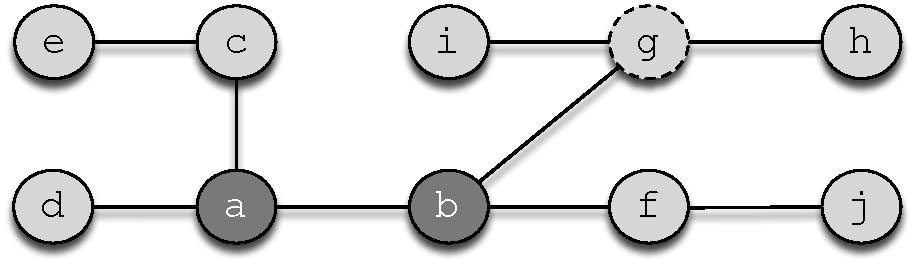
\includegraphics[scale=0.51]{figs/example4.pdf}
%\includegraphics[scale=0.51]{figs/example2.pdf}
\caption{Example power system graph. PMU nodes ($a,b$) are indicated with darker shading. Injection nodes have solid borders while zero-injection nodes  ($g$) have dashed borders.}
\label{fig:example}
\end{figure}

Using the same notation as Brueni and Heath \cite{Brueni05}, we define two $\Gamma$ functions. For $v\in V$ let $\Gamma(v)$ be the set of $v$'s neighbors in $G$, and $\Gamma[v] = \Gamma(v)\cup \{v\}$. 
% Since neighbor relationships are symmetric, $u\in\Gamma(v)\Rightleftarrow v\in\Gamma(u)$. 
A PMU placement $\Phi_G \subseteq V$ is a set of nodes at which PMUs are placed,
%We use the definition of a PMU placement from Brueni and Heath \cite{Brueni05}: a PMU cover, $\Phi$, is a subset of $V$ in which PMUs are placed such that all $v \in V$ and all $(u,v) \in E$ observed.
and $\Phi^R_G\subseteq V$ is the set of observed nodes for graph $G$ with placement $\Phi_G$ (see definition of observability below). %For convenience, we let $\Phi^R$ represent the observed nodes for graph $G$.
$k^* = \min \{|\Phi_G|:\Phi^R_G=V\}$ denotes the minimum number of PMUs needed to observe the entire network. Where the graph $G$ is clear from the context, we drop the $G$ subscript.
%Finally, $m$ is a constant corresponding to a graph $G=(V,E)$ such that $m < |V|$. 

%We let $\Phi^-$ represent the observed edges and $\Phi^R$ represent the observed nodes.
%All notation used in this document is shown in Table \ref{tab:notation}.

For convenience, we refer to any node with a PMU as a \emph{PMU node}. Additionally, for a given PMU placement we say that set $W\subseteq V$ is observed if all nodes in $W$ are observed, and if $W=V$ we refer to the graph as \emph{fully observed}. 


%%%%%%%%%%%%%%%%%%%%%%%%%%%%%%%%%%%%%%%%%%%%%%%%%%%%%%%%%%%%%%%%%%%% BEGIN COMMENT %%%%%%%%%%%%%%%%%%%%%%%%%%%%%%%%%%%%%%%%%%%%%%%%%%%%%%%%%%%%%%%%%%%%%%%%%%%%%%%%%%%%%%%%%%%%%%%%%%%%%%%%%%%%%%%%
\begin{comment}
\begin{table}[t]
\begin{center}
\begin{tabular}{l l} 
\hline \hline
   	{\bf Notation} & {\bf Meaning} \\
		  \hline 
		  	$G$ &  undirected graph $(V,E)$ where each $v \in V$ is a bus and each \\
				&  $(u,v) \in E$ is a transmission line connecting $u$ and $v$\\
			$\Gamma(v)$ & $\{u \in V$ $|$ $(u,v) \in E \}$ \\ 
			$\Gamma[v]$ & $\Gamma(v) \cup \{v\}$ \\
 		 	$n$ & $|V|$ \\
			$\Phi$ & a subset of $V$ in which PMUs are placed such that all \\ 
				   & $v \in V$ and all $(u,v) \in E$ observed  \\
			$\Phi^R$ & set of observed nodes \\
			$\Phi^-$ & set of observed edges \\
			\hline \hline
	\end{tabular}
	\end{center}
\caption{Notation Table}
\label{tab:notation}
\end{table}
\end{comment}
%%%%%%%%%%%%%%%%%%%%%%%%%%%%%%%%%%%%%%%%%%%%%%%%%%%%%%%%%%%%%%%%%%%% END COMMENT %%%%%%%%%%%%%%%%%%%%%%%%%%%%%%%%%%%%%%%%%%%%%%%%%%%%%%%%%%%%%%%%%%%%%%%%%%%%%%%%%%%%%%%%%%%%%%%%%%%%%%%%%%%%%%%%

\subsection{Observability Rules}
\label{subsec:observe}

We use the simplified observability rules elegantly formulated by Brueni and Heath \cite{Brueni05}.  We restate the rules here:  %which we restate here:  %For completeness, we restate the rules here:
%We use the simplified observability rules elegantly stated by Brueni and Heath \cite{Brueni05}, which we restate here:  %For completeness, we restate the rules here:
\begin{enumerate}
	
	\item {\bf Observability Rule 1 (O1)}.  {\it If node $v$ is a PMU node, then $\Gamma[v]$ is observed. Formally, if $v \in \Phi_G$, then $\Gamma[v] \subseteq \Phi^R_G$. }

	\item {\bf Observability Rule 2 (O2)}. {\it If a zero-injection node, $v$, is observed and  $\Gamma(v)\backslash\{u\}$ is observed for some $u\in\Gamma(v)$, then  $\Gamma[v]$ is observed.
	Formally, if $v \in \Phi^R_G \cap V_Z$ and $|\Gamma(v) \cap (V - \Phi^R_G)| \leq 1$, then $\Gamma[v] \subseteq \Phi^R_G$. }

\end{enumerate}

Consider the example in Figure \ref{fig:example}, where the shaded nodes are PMU nodes and $g$ is the only zero-injection node. 
%{\footnote {\small For all power system graphs shown in this document zero-injection nodes have a dashed border and injection nodes have a solid border.}}
Nodes $a-d$ are observed by applying O1 at the PMU at $a$, and nodes $a,b,f$ and $g$ are observed by applying O1 at $b$. 
$e$ cannot be observed via $c$ because $c$ does not have a PMU (O1 does not apply) and is an injection node (O2 does not apply). % so $e$ cannot be observed via $c$, which is its only neighbor. 
%$c$ does not have a PMU (O1 does not apply) and is an injection node (O2 does not apply), so $e$ cannot be observed via $c$, which is its only neighbor. 
Similarly, $j$ is not observed via $f$. Finally, although $g \in V_Z$, O2 cannot be applied at $g$ because $g$ has two unobserved neighbors $i,h$, so they remain unobserved.

Since O2 only applies with zero-injection nodes, more nodes are likely observed when nodes are zero-injection. For example, consider the case where $c$ and $f$ are {\em zero-injection} nodes. $a-d$, $g$ and $f$ are still observed as before, as O1 makes no 
conditions on the node type. Additionally, 
since $c,f \in V_Z$ and each has a single unobserved neighbor,  we can apply O2 at each of them to observe $e,j$, respectively. % making $e$ and $j$, respectively, observed.   
We evaluate the effect of increasing the number of zero-injection nodes on observability in our simulations (Section \ref{subsec:zero}).

%Finally, O2 can be applied at $e$ because $e \in V_Z$, $e$ is observed, and all of $e$'s neighbors except $i$ are observed. As a result, $i$ becomes observed. 
%Note that O2 cannot be applied at $f$ because $f$ has two unobserved neighbors. %This leaves $g$ and $h$ as the only two unobserved nodes in this example. 

%\begin{figure*}[t]
%  \begin{center}
%    \fbox{\subfigure[Case O1]{\label{fig:s1}\includegraphics[scale=0.28]{figs/s1.pdf}}}
%    \fbox{\subfigure[Case O2]{\label{fig:s2}\includegraphics[scale=0.28]{figs/s2.pdf}}} 
%  \end{center}
%	\caption{Rule Set 2} 
%  \label{fig:ruleset2}
%\end{figure*}




\subsection{Cross-Validation Rules}
\label{subsec:xval-rules}

% If phasor measured by 2 or more PMUs
From Vanfretti et al. \cite{Vanfretti10}, PMU measurements can be cross-validated when: (1) a 
voltage phasor of a non-PMU bus can be computed by PMU data from two different buses or (2) the current phasor of a transmission line can be computed from PMU data from two different buses. 
%Note that Vanfretti et al. \cite{Vanfretti10} use the term ``redundancy'' instead of cross-validation.  
{\footnote {\small  Vanfretti et al. \cite{Vanfretti10} use the term ``redundancy'' instead of cross-validation. }}  
Although it is the PMU data that is actually being cross-validated,
for convenience, we say a PMU is cross-validated. 
A PMU is \emph{cross-validated} if one of the rules below is satisfied \cite{Vanfretti10}: 
\begin{enumerate}
	
	\item {\bf Cross-Validation Rule 1 (XV1)}.  {\it If two PMU nodes are adjacent, then the PMUs cross-validate each other. % (Figure \ref{fig:validate}(a)). 
	Formally, if $u, v \in \Phi_G$, $u \in \Gamma(v)$, then the PMUs at $u$ and $v$ are cross-validated.}

	\item {\bf Cross-Validation Rule 2 (XV2)}. {\it If two PMU nodes have a common neighbor, then the PMUs cross-validate each other. % (Figure \ref{fig:validate}(b)). 
	Formally, if $u, v \in \Phi_G$, $u\neq v$ and $\Gamma(u)\cap\Gamma(v)\neq\emptyset$, then the PMUs at $u$ and $v$ are cross-validated.}
\end{enumerate}
In short, the cross-validation rules require that {\em the PMU is within two hops of another PMU}.
For example, in Figure \ref{fig:example}, the PMUs at $a$ and $b$ cross-validate each other by XV1. 

XV1 derives from the fact that both PMUs are measuring the current phasor of the transmission line connecting the two PMU nodes.  XV2 is more subtle.  
Using the notation specified in XV2, when computing the voltage phasor of an element in $\Gamma(u)\cap\Gamma(v)$ the voltage equations include variables to 
account for measurement error (e.g., angle bias) \cite{Vanfretti-thesis}. %\cite{Vanfretti10}.
When the PMUs are two hops from each other, there are more equations than unknowns, allowing for measurement error detection. 
Otherwise, the number of unknown variables exceeds the number of equations, which eliminates the possibility of detecting measurement errors \cite{Vanfretti-thesis}.
%Otherwise, the number of unknown variables grows faster than the number of equations, which eliminates the possibility of detecting measurement errors \cite{Vanfretti-thesis}.

%XV1 derives from the fact that both PMUs are measuring the current phasor of the transmission line connecting the two PMU nodes.  XV2 is more subtle.
%Using the notation specified in XV2, when computing the voltage phasor of an element in $\Gamma(u)\cap\Gamma(v)$ the equations include variables to account for measurement error (e.g., angle bias).
%%In order to account for measurement error, the equations used to compute the voltage phasor of the neighbor node shared by the PMU nodes include varialbes to account
%%for measurement error. Computing the voltage phasor of the neighbor node shared by the two PMU nodes
%%When computing the voltage phasor of the common neighbor node shared by the PMU nodes the equations include variables to account for measurement error (e.g., angle bias).
%When the PMUs are two hops from each other, there are more equations than unknowns, allowing for measurement error detection.
%Otherwise, the number of unknown variables exceeds the number of equations, which eliminates the possibility of detecting measurement errors \cite{Vanfretti-thesis}.
%Otherwise, the number of unknown variables grows faster than the number of equations, which eliminates the possibility of detecting measurement errors \cite{Vanfretti-thesis}.






\section{Algorithms}
\label{sec:algs}

We propose a set of algorithms, collectively referred to as \mdrs, that make multicast trees robust to link failures.  
\footnote{The name \mdr is inspired by Johnny Appleseed, the famous American pioneer and conservationist known for planting apple nurseries and caring for its trees. }
\mdr runs at the OpenFlow controller with the goal of minimizing packet loss associated with link failures while ensuring that end-to-end delay requirements are satisfied.
\mdr divides into three parts: %each presented in detail in this section: 
\begin{enumerate}
	\item {\bf \pcnt algorithm: monitor and quickly detect link failures} when and where they occur inside the network (Section \ref{subsec:pcnt}).
	
	\item {\bf Precompute backup trees} that are amenable to fast installation.  In Section \ref{subsec:min-control} we formulate a new problem, \mcs, that aims to compute backup trees that
	reuse primary tree edges, prove \mc is at least NP-hard, and provide an approximation algorithm for \mc called \steiners.
	%minimize control plane signaling overhead, prove \mc is at least NP-hard, and provide an approximation algorithm for \mc called \steiners.

	\item {\bf Fast install of pre-computed backup trees} by reusing existing forwarding rules installed in the network, sharing forwarding rules among backup trees with common links, and
	in some cases pre-installing forwarding rules before link failures occur (Section \ref{subsec:install-backups}).  
	The backup trees are computed using \steiner from part (2). \pcnts, from part (1), triggers the installation of a set of backup trees.

	 %backup tree installed and shown in Figure \ref{fig:intuition-example-t2}).
	
\end{enumerate}


%to make multicast trees robust to link failures by monitoring and detecting failed links, precomputing backup multicast trees, and efficiently installing backup multicast trees after a link failure.
%As input, \mdr is given an undirected graph containing OpenFlow switches; the set of all multicast trees ($T$); the set of all active multicast flows ($F$); the length of each sampling window, 
%$w$, used to monitor links and specified in units of time; and, for each multicast flow, a packet loss condition for each link the flow traverses. For now, we restrict packet loss conditions 
%to be threshold-based that indicate the maximum number of packets that can be lost over $w$ time units. 
%The output of \mdr is a new set of precomputed backup multicast trees installed in the network and a set of uninstalled multicast trees.   All $T_i \in T$ that use the failed link are uninstalled and we call each such $T_i$ a \emph{failed multicast tree}.
%%The set of installed MTs includes each $T_i \in T$ that does not use the failed link and a backup tree for any $T_i$ that does. %does use a failed link.

%{\it TODO: write overview that unifies packet loss and E2E delay.}






%\subsection{Link Failure Detection using OpenFlow}
%\label{subsec:detection}

%missing: (a) openflow match and action, (b) flow-level measurement or packet loss at links

In this section, we propose a simple algorithm (\fls), used by \mdrs, that monitors links \emph{inside} the network to detect any packet loss.  To help explain \fls,
we use the example scenario from Section \ref{subsec:scenario} and refer to a generic multicast tree with an upstream node, $u$, and downstream node, $d$.
%Our presentation of \fl is necessarily brief but we provide additional details in Appendix \ref{subsec:pcnt}.  

\fl is run at the OpenFlow controller and provides accurate packet loss measurements that are the basis for identifying lossy links.
Informally, a lossy link is one that fails to meet the packet loss conditions specified by the controller.  We refer to such a link as \emph{failed}.
Although \mdr is ultimately concerned with meeting the per-packet \emph{delay} requirements of PMU applications, 
we use  packet loss (as opposed to delay) as an indicator for a failed link because OpenFlow provides no native support for timers.

\fl has the same input as \mdrs, specified in Section \ref{subsec:mdr}.
The output of \fl is any link that has lost packets not meeting the packet loss condition of any multicast flow traversing the link. 
In the remainder of this document, we assume all flows are multicast and just use \emph{flow} to refer to a multicast flow, unless otherwise specified.

Recall from Section \ref{subsec:openflow} that each OpenFlow switch maintains a flow table, where each entry contains a match rule 
(i.e., an expression defined over the packet header fields used to match incoming packets) and action 
(e.g., ``send packet out port $2$''). For each packet that arrives at an OpenFlow switch, it is first matched to a flow entry, $e$, based on the packet's header fields; 
then $e$'s packet counter is incremented; and, lastly, $e$'s action is executed on the packet. 
\footnote{Not all switches are necessarily OpenFlow-enabled. In fact, we anticipate that in practice many switches will not support OpenFlow. \fl still works such scenarios, as long as 
the packet counts are taken at OpenFlow switches. For ease of presentation, this section assumes all switches are OpenFlow-enabled.}
\fl uses these packet counter values to compute per-flow packet loss between switches over $w$ time units. 

%pcount(upstream_switch,downstream_switchs,nw_src, nw_dst,window_size) or pcount(upstream_switch,downstream_switchs,flow,window_size) 
\fl uses the subroutine, \pcnts, to measure the packet loss between an upstream node ($u$) and one or more downstream nodes.  For simplicity, we assume only a single downstream node, $d$. 
\pcnt does so on a per-flow basis over a specified sampling window, $w$, 
where $w$ is the length of time packets are counted at $u$ and $d$. For each window of length $w$, \pcnt computes packet loss for a flow $f$, that traverses $u$ and $d$, using the following steps:
\begin{enumerate}
	\item 
	\textbf{At $u$, tags and counts all $f$ packets}.  
	We assume, before any changes are made, $u$ uses flow entry $e$ to match and forward $f$ packets.
	\pcnt creates a new flow entry, $e'$, that is an exact copy of $e$, except that $e'$ embeds a unique identifier (i.e., the tag) in the packet's VLAN Id field.  Let this identifying number
	be $1111$.
	$e'$ is installed with a higher priority than $e$.  In OpenFlow, each flow entry has a corresponding priority specified upon its installation.
	%OpenFlow switches order flow entries based on their specified priority.  
	Incoming packets are matched against flow entries in priority order, with the first matching entry being used. 
	Thus, setting a higher priority for $e'$ than $e$, ensures that $u$ writes $1111$ in the VLAN Id field of all $f$ packets when $e'$ is installed.

	\item
	\textbf{Counts all tagged $f$ packets received at $d$.} \pcnt does so by installing a new flow entry at $d$, $e''$, that matches packets with VLAN Id equal to $1111$. 
	%in based on the VLAN tag applied at $u$.  

	\item 
	\textbf{After $w$ time units, turns tagging off at $u$.} To do so, \pcnt simply switches the priority of $e'$ and $e$ at $u$. 
	\footnote{\xxn{Unfortunately, OpenFlow does not allow a flow's priority to be modified.  As a workaround, we install a copy of $e$ called $e_c$.  We ensure that $e_c$ is given 
	a higher priority than $e'$.  Finally, we delete flows $e$. }}

	\item
	\textbf{Queries $u$ and $d$ for packet counts.} 
	Specifically, the controller uses the OpenFlow protocol to query $u$ for $e'$'s packet count value and $d$'s packet count value for $e''$.
	To ensure that all in-transit packets are considered, \pcnt waits ``long enough'' for in-transit packets to reach $d$, before reading $d$'s packet counter 
	(e.g., time proportional to the average per-packet delay between $u$ and $d$).

	\item
	\textbf{Garbage collection.}
	As a cleanup step delete $e'$ at $u$ and $e''$ at $d$.

	\item 
	\textbf{Computes packet loss.}
	The controller computes packet loss by simply subtracting $e'$'s packet count from $e''$'s. 

\end{enumerate}
In practice, \pcnt executes step (2) before step (1) to ensure that $u$ and $d$ consider the same set of packets.

%execute the actions specified by the first flow entry matching the packet's header

\pcnt introduced minimal overhead.  At $u$ and at each downstream counting switch, a copy of the flow entry corresponding to $f$ is required.  
However, these copies only persist during the duration of each \pcnt interval.


In the Figure \ref{fig:intuition-example} example, the controller uses \fl to measure the packet loss for the $a,\{e,f\}$ flow.  
We assume for link $(b,c)$ and the $a,\{e,f\}$ flow, \fl is given a maximum packet loss threshold of $10$ packets over $w$ time units.
For each sampling window of $w$ time units, \pcnt instructs $b$ to tag and count all packets corresponding to $a,\{e,f\}$. 
At the same time, $c$ is instructed by \pcnt to count the $a,\{e,f\}$ packets tagged by $b$. Then, the controller uses the OpenFlow protocol to query the packet counter values for $a,\{e,f\}$
at $b$ and $c$.  When $(b,c)$ fails, the packet counter at $c$ for $a,\{e,f\}$ no longer increments, causing a violation of $a,\{e,f\}$'s packet loss threshold for $(b,c)$.

\xxx{describe how pcount can reduce the number of necessary measurement points}

%As specified, \fl measures packet loss for each \emph{multicast flow} at each link.  These flow-level measurements may obfuscate aggregate link-level packet loss. For this
%reason, we plan to extend \fl to group flows together to enable \emph{aggregate} packet loss measurements. 
%Because OpenFlow provides native support for grouping flows and maintains packet counters for each 
%group, \fl can be easily extended to group and count packets for any subset of multicast flows traversing the same switch.


\pcnts's approach for ensuring consistent reads of packet counters bears strong resemblance to the idea of \emph{per-packet consistency} introduced by Reitblatt et al.~\cite{Reitblatt11}.
Per-packet consistency ensures that when a network of switches change from an old policy to a new one, that
each packet is guaranteed to be handled exclusively by one policy, rather than some combination of the two policies.  In our case, we use per-packet consistency to ensure that when \pcnt reads
$u$ and $d$'s packet counters, exactly the same set of packets are considered, excluding, of course, packets that are dropped at $u$ or dropped along the path from $u$ to $d$. 

\xxn{\fl is fast because it detects link failures inside the network, rather than on an end-to-end basis.  We plan to quantify how much faster \fl is than end-to-end link failure detection 
techniques.  In addition, \fl allows for link failures to be localized, whereas end-to-end techniques may not provide the necessary insight to identify and isolate the faulty link.
}

%\xxn{Advantage of in-network detection is not just the speed but also it allows us to localize the problematic links.  End-to-end detection does not provide this insight, or at least
%not as directly.}



\xxx{ $e$ matches using tuple $(src,dst,VLAN)$}

\subsubsection{\pcnt Evaluation}

\xxxx{move this section, possibly the E2E discussion to the related work section.}

{\bf Detection using end-to-end measurements.}
An alternative approach to link failure detection is to use end-to-end probes to infer packet loss rates of individual links. C\`{a}ceres et al. \cite{Caceres99} propose a maximum likelihood estimator
for loss rates of internal links based on losses observed by multicast receivers. Their model uses the inherent correlation of packet loss across multicast receivers to improve accuracy 
of their packet loss estimates.  Although impressive accuracy results are reported, the authors' simulations show that about $2000$ end-to-end probe messages are required for packet loss
estimates to converge on the true underlying packet loss rate \cite{Caceres99}.  In our problem setting, packet loss needs to be detected over small windows of time and, unfortunately,
$2000$ messages would correspond to too larger a window of time. For this reason, we deem solutions based on end-to-end measurements a poor match for our problem domain.

{\bf 7/20/13 writing from grant about plans for evaluation.}
To date, we have implemented \pcnt in the POX OpenFlow controller using the Mininet emulator and plan to further evaluate \pcnt by using our POX-based implementation to work with real
OpenFlow switches.  To provide a point of reference, we plan to implement and measure a simple SNMP-based approach for detecting link-level packet loss.  We will quantify the error rate of \pcnt 
and the SNMP-based approach as a function of the sampling window size.  We will also quantify the detection time for \pcnt and the SNMP-based approach as a function of window size. We believe our measurement study will show \pcnt  provides accurate and fast packet loss detection across all sampling window sizes, making it a superior approach for ultra- reliable data dissemination in smart grid networks


%%%%%%%%%%%%%%%%%%%%%%%%%%%%%%%%%%%%%%%%%%%%%%%%%%%%%%%%%%%%%%%%%%%%%  END OF DETECTION SECTION %%%%%%%%%%%%%%%%%%%%%%%%%%%%%%%%%%%%%%%%%%%%%%%%%%%%%%%%%%%%%%%%%%%%%%%%%%%%%%%%%%%%%%%%%%








%\subsection{Multicast Implementation} 
\label{subsec:basic}

In keeping with its role as a general framework that provides primitives for programmable networks, OpenFlow does not explicitly provide an implementation for multicast. 
Instead, we design our own multicast implementation called \bases.  \base assign a multicast IP address to each multicast group and use
this address to setup the flow tables at the multicast tree switches.  
  \footnote{Because multicast group membership is static for power grid applications (Section \ref{subsec:pmu-requirements}, 
  we simply determine the members of each multicast group by reading their static assignment from a text file.  Note that if dynamic group membership were to be required, we could 
  replace this static policy using a protocol like IGMP. }

After the controller computes a multicast tree (described in Section \ref{subsec:min-control}), $T_i = (V_i,E_i,r,S)$, \base installs a flow entry at each switch in $V_i$. The flow entry
matches packets using the group's multicast address (all other field are left as wildcards) and sends a copy of each packet out the ports corresponding to the switch's 
outgoing links in $E_i$. If a switch in $E_i$ is adjacent to a downstream host, $h_j$, in the multicast group, then the flow entry rewrites the destination layer 2 and 3 addresses of the 
packet copy sent to $h_j$ to $h_j$'s layer 2 and 3 addresses.
\footnote{Our initial plan was to use the group table abstraction described in the OpenFlow 1.1 specification \cite{OpenFlowSpec1.1} to implement multicast but, unfortunately,
as of the writing of this paper, this feature is not yet supported by the POX controller \cite{Pox} used to implement our algorithms and 
the Mininet emulator \cite{Lantz10} used in our simulations.}

% (1) mcast group assigned mcast address, (2) After mcast tree computed for mcast group, use dst address to match packets at each switch.  packets fwded out the ports corresponding to
%  tree links, rewrite address at leaf switches.  (action applied for leaf's outport)

%those of its adjacent downstream host. (these fields were previously populated with the multicast addresses).




%Another way to implement multicast in OpenFlow is to leverage existing IP multicast protocols as detailed by Kotani et al. \cite{Kotani12}.  
%In this approach, the controller assigns a unique group ID to each multicast tree and creates a group table entry, that uses the group ID, at each switch along the multicast tree.  
%Meanwhile, the sender and its first-hop switch use IGMP to set up and manage the controller-generated group IDs. Finally, the sender embeds the group ID in each multicast packet's destination 
%field, allowing for each switch in the multicast tree to identify and forward multicast packets appropriately. 



\subsection{Computing Backup Trees}
\label{subsec:min-control}

\mdr pre-computes backup trees to install after \pcnt detects a link failure.  Here we present a new problem, \mcs, and approximate solution to \mcs, called \steiners, that aim to facilitate fast
recovery by computing backup trees that maximize the number of edges common between each backup tree and its primary tree.  This reuse of primary tree edges speeds recovery from link
failures because, in SDN, this reduces the number of new flow table entries that need to be installed in the network in response to a link failure.

\mdr uses \steiner as a part of system initialization where a set of backup trees are computed for each network link, $l$; \mdr computes a single backup tree for each primary tree using $l$. 
Additionally, \steiner is used after a set of backup trees, $\hat{T}^l$, are installed in response to a link failure.  For each newly installed tree $\hat{T}^l_i \in \hat{T}^l$, \mdr computes 
a backup tree for each link in $\hat{T}^l_i$.
%recovery by minimizing control overhead (i.e., number of new flow table entries) required to install backup trees.  

%In SDNs, reusing forwarding rules which under SDN reduces the number of new flow table entries required to install backup trees.  

%\mdr uses \steiner in two scenarios. One, as a part of system 
%initialization where a set of backup trees are computed for each network link, $l$; \mdr computes a single backup tree for each primary tree using $l$.  Two, \mdr triggers the execution of 
%backup tree computations after backup trees, $T_l$, are installed in response $l$'s failure. \mdr recomputes backup trees for all primary trees as opposed to only the newly install $T_l$ trees.
%The motivation for recomputing all backup trees is that the network state -- the set of installed forwarding rules -- is 
% the entire computation (as opposed to only computing backup trees for the newly installed
%Tl trees): for each network link, l, Appleseed computes a backup MT for each MT that would be affected if l failed. Appleseed recomputes all backup MTs because installing the Tl MTs changes how flows are distributed and processed inside the network and, as a result, may adversely affect flows processed by MTs other than those in Tl. In other words, backup MTs computed before l fails may become stale when the Tl MTs are installed since the algorithms used to compute them considered an old network state in their optimization. 

\subsubsection{\mcn Problem}
\label{subsubsec:min-control}

% Existing Outline:  (a) control overhead definition + example, (b) multiple PTs need entry for each tree (c) benefits of reducing control overhead, (d) problem definition, (e) NP-hard
% Revised Outline:  (a) informal control overhead + benefits, (b) control overhead definition, (c) example, (d) problem statement, (e) NP-hardness outline
%control overhead definition + example, (b) multiple PTs need entry for each tree (c) benefits of reducing control overhead, (d) problem definition, (e) NP-hard 
% make sure handle 1 message per flow assumptio

\mc considers backup trees that maximize reuse of primary tree edges.  Recycling primary tree edges allows the SDN controller, when generating the forwarding rules for multicasting 
packets using the backup tree, to use primary tree rules already installed in the network rather than install new ones.
%Recycling primary tree rules reduces the number rule installation messages, referred to as control messages, the controller must send network switches. 
This speeds recovery in cases where backup trees are installed \emph{after} a link failure is detected and reduces the number of flow table entries pre-installed at switches (control state) 
when backup trees are installed \emph{before} a link failure occurs.  
Reducing control state is especially important with OpenFlow because OpenFlow switches can only store a limited number of flow table entries (see Section \ref{subsec:openflow}).
\footnote{Following from our assumption that a single link fails at-a-time, \mc assumes that all other links besides the failed one, $l$, satisfy packet loss requirements. }
%\footnote{Our \mc description implies that all other links besides the failed one, $l$, satisfy packet loss requirements. This follows from our assumption that only a single link fails at-a-time.}

For the primary tree $T^l_i = (V^l_i,E^l_i,r,S)$ and its backup $\hat{T}^l_i=(\hat{V}^l_i,\hat{E}^l_i,r,S)$, we define a binary variable $c_v^l$ for all $v \in \hat{V}_i^l$. 
If $v$ has exactly the same predecessors (outgoing edges) in $T^l_i$ and $\hat{T}^l_i$, then $c_v^l$ takes value $0$.  Otherwise, $c_v^l=1$.  
%Using  $c_v^l$, define: %Define multicast recycling, for the $T^l_i$,$\hat{T}^l_i$ pair as:
For the $T^l_i$,$\hat{T}^l_i$ pair define:
\begin{eqnarray}
\label{eqn:control-overhead}
 C_i^l &=&  \sum_{\forall v \in \hat{V}_i^l} c_v^l 
\end{eqnarray}
For our purposes, $C_i^l$ is the number of new rules (i.e., non-recycled primary tree rules) needed to install $\hat{T}^l_i$.

Consider the example in Figure \ref{fig:intuition-example} where $(g,l)$ fails. The green backup tree, $\hat{T}_b$, shown in Figure \ref{fig:intuition-example-t2}, has $C_b =2$ because 
a new forwarding rule is required at $b$, and $f$ to account for the new outgoing links at each node. $\hat{T}_c$, in blue, has
only one link, $(m,l)$ not in $\hat{T}_c$'s primary tree. As a result, $C_c =3$.

Our \mc problem definition below references a modified version of the Steiner tree problem, called the \arbor problem \cite{Charikar98}. As input \arbors, is given 
a directed graph $G=(V,A)$, a root vertex $r$, and a set of terminals, $S$. An arborescence is defined as a tree directed away from $r$ that spans $S$.  \arbor aims to find a minimum cost 
arborescence, called a Steiner arborescence or directed Steiner tree. We denote $SA_i(G) = (V,E,r,S)$ as the $ith$ Steiner arborescence computed over directed graph, $G$, .

We use the following formulation for the \mc problem: 
\begin{itemize}

	%\item  \underline{Input}: $(G,T,l)$ where $G=(V,E)$ is directed graph, $T=\{T_1,T_2, \dots T_m\}$ where each $T_i \in T$ is a primary tree, and $l \in E$.
	\item  \underline{Input}: $(G,T^l,l,\alpha)$ where $G=(V,E)$ is a directed graph, $T^l=\{T_1^l,T_2^l, \dots T_k^l\}$ where each $T_i^l \in T^l$ is a primary tree that uses $l$, 
	$l \in E$, and $\alpha \geq 1$. 
	%computed using the directed Steiner tree approximation algorithm described by Charikar et al. \cite{Charikar98}, and $l \in E$.


	\item \underline{Output}: A backup tree for each primary tree using $l$. This set of backup trees, $\hat{T}^l = \{\hat{T}^l_1,\hat{T}^l_2,\dots,\hat{T}^l_k\}$:
		\begin{equation}
		\label{eqn:mc-obj-function}
		\begin{aligned}
			& {\text{minimize}}
			& & \sum_{1 \leq i \leq k} C^l_i \\
			& \text{subject to}
			& & w(\hat{T}^l_i) \leq \alpha \cdot w(SA_i(G')), \;  \forall \hat{T}^l_i \in \hat{T}^l \\
		\end{aligned}
		\end{equation}
		where $G'=(V',E')$ such that $E' = E - \{l\}$ and $w(\hat{T}^l_i)$ is the sum of $\hat{T}^l_i$'s link weights.	
		\footnote{We assume $\hat{T}^l_i$, satisfies all per-packet delay and loss requirements if $l \notin \hat{T}^l_i$ and $w(\hat{T}^l_i) \leq \alpha \cdot w(SA_i(G'))$}

\end{itemize}   % (a) assumes all other links up, (b) C^l defined between pt and bt, point shall revisit later in approx, (c) \alpha keeps tree from growing too larger
The objective function maximizes the reuse of primary tree edges, while $\alpha$ bounds how large the backup tree can grow as consequence of minimizing $C^l_i$.  When applied to our
problem scenario this formulation reduces the number of installation rules by reusing rules already installed in the network, under the constraint that the 
backup tree does not become too large to meet the end-to-end latency requirements. 
By defining $G'$ as a copy of $G$ with the failed link removed from $G$, we are assuming that all links in $G$ besides $l$ are operational.  For
our purposes, this amounts to assuming that all non-$l$ links have packet loss rates less than their threshold. %below the satisfy their packet loss rate condition.  

Notice that we have defined $C^l_i$ in Equation \ref{eqn:control-overhead} on a per-backup tree basis where for backup tree $\hat{T}^l_i$, $C^l_i$ is a relationship defined strictly between 
$\hat{T}^l_i$ and its primary tree $T^l_i$ (there are no constraints specified across any other primary or backup tree). 
%\footnote{This simplification is reasonable for our OpenFlow-based application of \mcs. In cases where multiple backup trees require a new forwarding rule at the same switch, $v$, a separate
%forwarding rule must be installed (even if these backup trees have exactly the same predecessors at $v$) for each of these backup trees because under our multicast implementation, 
%\bases, each forwarding rule matches packets using the tree's multicast address. }
As a result, the globally optimal solution for \mc  (i.e., the optimal set of backup trees for a single link)  can be found by computing the optimal backup for each primary tree in isolation
and then taking the union of these solution We shall revisit this important property when describing our approximation algorithm for \mcs.

\begin{theorem}
\label{thm:mc-npc}
\mc is at least NP-hard.
\end{theorem}
\begin{proof}
The details of our proof can be found in Appendix \ref{sec:mc-npc}. This proof shows that \mc is NP-hard even when considering just a single backup tree.  The proof demonstrates that
in some cases an optimal solution to \mc requires a solution to \arbors, a problem known to be NP-hard.  This proves \mc is NP-hard when considering a single backup tree and therefore
the general \mc problem for $k$ backup trees must at least be NP-hard. 
\end{proof}


%to derive a globally optimal solution for \mcs.  
%Notice that we have defined the control overhead as the difference between the directed edges from the backup tree and its corresponding primary tree.  This formulation
%is convenient because for a given link, $l$, we can solve \mco seperately for each directed tree using $l$ and then simply take the union of these solutions to derive a 
%globally optimal solution for \mc (for $l$).  




\subsubsection{\steinern Approximation Algorithm}
\label{subsubsec:steiner-approx}

\steiner is a simple approximation algorithm for \mc that manipulates link weights to encourage each backup tree to reuse primary tree edges.
For each link $l$,  \steiner separately computes a backup tree for primary tree using $l$ and then returns the union of these computed trees. 

%Our \mc approximation algorithm, \steiners, computes each backup tree for link $l$ separately and then returns the union of these computed trees. 
%\steiner manipulates link weights to encourage each backup tree to reuse primary tree edges. 

%\steiner leverages the \arbor approximation algorithm from Charikar et al. \cite{Charikar98}.  Their approximation algorithm computes a bunch: a subgraph 
%formed by taking the shortest path from the root to an intermediate vertex, $j$, and the union of shortest paths from $j$ to the terminal nodes.  
\steiner leverages the $\sqrt{s}$ \arbor approximation, where $s$ is the number of terminal nodes, from Charikar et al. \cite{Charikar98}. Their approximation algorithm computes bunches, 
where a \emph{bunch} is a subgraph formed by taking the shortest path from the root to an intermediate vertex, $i$, and the union of shortest paths from $i$ to the terminal nodes.  
The algorithm produces the bunch with best \emph{density} -- density is the average cost of connecting a terminal node with the root -- as its approximation.   The lowest density bunch can 
easily be computed in polynomial time: a brute-force approach that tries all possible nodes as the intermediate vertex yields an $O(ns^2 \log s)$ time algorithm. 
%where $s$ is the number of terminal nodes.  The authors prove this is a $\sqrt{s}$ approximation.


%\steiner leverages the \arbor approximation algorithm from Charikar et al. \cite{Charikar98}.  Their approximation algorithm recursively finds ``bunches'', where a bunch is a subgraph 
%formed by taking the shortest path from the root to an intermediate vertex, $j$, and the union of shortest paths from $j$ to a subset of the terminal nodes.  
%Th%e overall solution is the union of each bunch.  %We denote $B_i(G) = (V,E,r,S)$ as the $ith$ Steiner arborescence computed over directed graph, $G$, using this algorithm.
%\footnote{In our work, the initial set of primary trees (i.e., the primary trees used before any link failures) are computed using the Steiner arborescence approximation from \cite{Charikar98}.}

%Our approximation algorithm for \mc solves computes for each $T_i^l \in T^l$ and then returns the union of these results. 
%We leverage the Steiner arborescence approximation described in \cite{Charikar98} to approximate \mcos.  Abusing notation, we refer to the \mco primary tree as $T^l$ and its backup as $\hat{T}^l$.  

Given $(G,T^l,l,\alpha)$, for each $T_i^l \in T^l$ \steiner uses the following two-step procedure to compute $\hat{T}^l_i$:
\begin{enumerate}
	
	\item Make a copy of $G$ called $G'=(V',E')$ and remove $l$ from $E'$.  Set the link weight of each $e \in T^l_i$ to $0$ and the link weight of $e \notin T^l_i$ to $1$. 

	\item Run the \arbor approximation, using the brute-force approach described above, over $G'$ and set $\hat{T}^l_i$ to be the result.
	If $\hat{T}^l_i$ satisfies the Equation \ref{eqn:mc-obj-function} constraint, return $\hat{T}^l_i$ as the solution.  Otherwise, return False. 
	%Otherwise, compute the backup tree from scratch -- run the \arbor approximation 
	%over a copy of $G$ that uses $G$'s original link weights and has link $l$ removed -- and return this result.

\end{enumerate}
Setting the primary tree link weights to $0$ in Step (1) allows the \arbor approximation algorithm to use any primary tree edge without penalty (i.e., adding cost to the 
backup tree) and so encourages reusing primary tree edges.  If \steiner returns False in Step (2) either $\alpha$ must be made larger or a new multicast tree should be computed from
scratch that satisfies the tree size constraint.

In Figure \ref{fig:intuition-example}, \steiner uses $f$ as the the intermediate node for $\hat{T}_b$, yielding density of $2$ (the cost of connecting terminals $p$,$q$,$r$, and $s$ to the 
root is $2$).   The bunch for $\hat{T}_c$ is formed using $m$ as the intermediate node with density $0.4$: the cost of connecting $r$ and $s$ to the root is $1$ and $t$,$u$, and $v$ connect
with the root at $0$ cost. 






\subsection{Installing Backup Trees}
\label{subsec:install-backups}

We are now ready to describe the last part of \mdrs, installing backup trees.  %(like the ones computed by \steiners): \pre and \posts.  
Installing a backup tree is a two-step process. First, the flow entries that forward packets along the backup tree are generated.  Second, the 
controller signals the necessary switches to install the generated forwarding rules.  Here we introduce two such installation algorithms, \pre and \posts.
Both algorithms compute forwarding rules for a single backup tree at-a-time and so
our description of each algorithm (with some abuse of notation) refers to a generic primary tree, $T^l = (V^l,E^l,r,S)$, and its backup tree for $l \in E^l$, $\hat{T}^l=(\hat{V}^l,\hat{E}^l,r,S)$.  

{\bf \post \textsc{Algorithm.}}
First, \post determines which nodes require a new forwarding rule. % to install the backup tree.
 In cases where $\hat{T}^l$ and $T^l$ use exactly the same outgoing links of a common node, $u$, we say
$\hat{T}^l$ can ``reuse'' $T^l$'s forwarding rule at $u$;  since $T^l$'s forwarding rule is already installed at $u$, no new forwarding rule (for $\hat{T}^l$) needs to be installed. % at $u$.
Forwarding rules are only required at any $v \in \hat{V}^l \setminus V^l$ and at each $v \in V^l \cap \hat{V}^l$ with different outgoing links in $\hat{T}^l$ and $T^l$.  We refer to this
set of nodes as $B^l$. 

Consider $T_b$ and $\hat{T}_b$ in the Figure \ref{fig:intuition-example} example. Because $T_b$ and $\hat{T}_b$  share the same outgoing links at $l$ and $k$
$\hat{T}_b$ can reuse $T_b$'s flow entry at each of these nodes, whereas new forwarding rules are required at $b$ and $f$.

%Later in the document, we refer to the flow entries generated by \base as \emph{basic} flow entries
Second, \post pre-computes a \emph{basic} flow entry for each $b \in B^l$.  Like the flow entries \base computes (see Section \ref{subsec:basic}), a basic flow
entry, for a multicast tree $T_i$ and $u \in V_i$, matches packets using $T_i$'s multicast address and has instructions to send matching packets out the correct ports at $u$. 
%The ports are correct if the outgoing links corresponding to $e_u$'s outports are in $T^l$.
Lastly, when $l$ fails, the \post signals each $b \in B^l$ to install the pre-computed basic flow rule.
%The nodes are signalled sequentially, in bottom-up order, starting
%with the most downstream node in $U$. Bottom-up signaling ensures that each $u \in U^l$ has a matching flow entry when $\hat{T}^l$ packets arrive.


%\begin{figure}
%  \centering
%   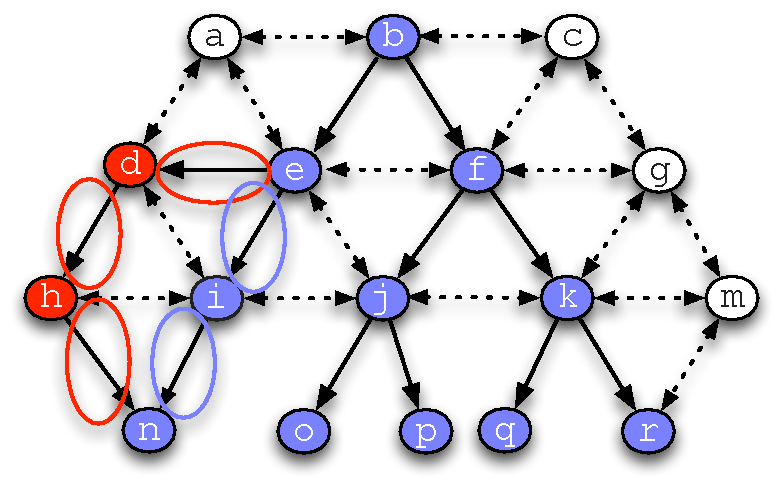
\includegraphics[scale=0.51]{figs/min-control-directed-example.pdf}
%\caption{Primary tree $T^l$ and backup tree, $\hat{T}^l$, where $l=(e,i)$. Edges unique to $T^l$ are circled in blue and unique $\hat{T}^l$ edges are circled in red. 
%$V^l \setminus \hat{V}^l = \{i\}$ and $\hat{V}^l \setminus V^l = \{d,h\}$. }
%\label{fig:min-control-example}
%\end{figure}


{\bf \pre \textsc{Algorithm.}}
\pre computes and installs backup tree flow entries \emph{before} a primary tree link, $l$, fails.  After $l$ fails, \pre signals the backup tree root
to install a forwarding rule that activates the backup tree.  We use the term ``activate'' to mean packets are multicasted using the backup tree rather than the primary tree.

%as opposed to \post that requires signaling multiple nodes to install a backup tree, \pre yields faster recovery than \posts. 

\pre cannot, without modifications, pre-install basic flow entries at all nodes because incorrect forwarding would result. Doing so at a node, $d$, common to the primary and backup tree
where the backup and primary tree have different outgoing links would either result in packets erroneously forwarded at $d$ using the backup tree before a link failure occurs or 
incorrectly forwarding packets using the primary tree after the link failure. 
We say that $d \in D^l$, where $D^l$ contains each node with one or more outgoing links in $T^l$ and one or more outgoing links in $\hat{T}^l \setminus T^l$.
Revisiting the Figure \ref{fig:intuition-example} example, installing a $\hat{T}_c$ forwarding rule at $g$ and $m$ before $(g,l)$ fails would be problematic for the reasons just described.

%Because $e$ has an outgoing link $(e,i) \in T^l$ and another outgoing link $(e,d)$ unique to $\hat{T}^l$,
%pre-installing $\hat{T}^l$'s flow entry at $e$ would cause incorrect forwarding for either $T^l$ or $\hat{T}^l$.  
%We say that $e \in D^l$, where $D^l$ contains each node with one or more outgoing links in $T^l$ and one or more outgoing links in $\hat{T}^l \setminus T^l$.

%{\it [TODO: Missing description of how root node is signaled to write the {\tt bid}. ]}

To address this issue, \pre assigns a unique \emph{backup tree id}, denoted {\tt bid}, to each backup tree.  For each $d \in D^l$, the flow entry matches and forwards packets
using the {\tt bid} value written in the {\tt dl\_src} field. When the backup tree $\hat{T}^l$ is activated, \pre writes the {\tt bid} in the
{\tt dl\_src} packet header field, indicating that these packets should be disseminated by $\hat{T}^l$ rather than $T^l$.
In more detail, \pre preinstalls and activates $\hat{T}^l$ using the following steps, where we assume $\hat{T}^l$ has {\tt bid=AA}:
\begin{enumerate}
	%\item Computes $D^l$.
	
	\item At each $d \in D^l$, \pre pre-installs a flow entry matching packets using $\hat{T}^l$'s multicast address, {\tt dl\_src = AA}, and wildcards for all other match fields. 
	%\footnote{We assume $T^l$ has multicast address \mdsts.}
	
	\item Preinstalls a basic flow entry at each $b \in B^l \setminus D^l$.

	\item When it is detected that $l$ fails, \pre installs a rule at the $\hat{T}^l$ root node that writes {\tt AA} in the {\tt dl\_src} header field of each $\hat{T}^l$ packet.
	%$e_r$ is given a higher priority than any other rule installed at $r$.
\end{enumerate}

For $\hat{T}_c$ in Figure \ref{fig:intuition-example}, \pre pre-installs a forwarding rule at $m$ that matches packets using $\hat{T}_c$'s {\tt bid}, {\tt CC}, and $T_c$'s multicast 
address.  After $(g,l)$ fails, \pre signals $c$ to write {\tt CC} in the {\tt dl\_src} header field of each $\hat{T}_c$ packet.  As a result, packets at $m$ are correctly forwarded to $l$,
$n$, and $t$.

{\bf Comparing \pre and \posts.}
Since \pre must signal only a single node, as opposed to multiple nodes with \posts, to install a backup tree, \pre is fast. However, \pres's speed comes at the cost of 
storing a potentially large number of flow entries at the switches, especially since \mdr computes, for each primary tree, a backup tree for each primary tree link. \post, on the other hand,
only installs backup tree flow entries after a link failure is detected.
These trade-offs are studied in Section \ref{sec:evaluation} using simulations.

%\post installs backup tree forwarding rules after a link failure is detected, while \pre installs backup tree flow entries before a link failure occurs. With \pres, the backup 
%trees are only activated -- by writing an identifier in each packet header signaling packets to be routed using the backup tree -- after the link failure is detected.

%\pre requires that only the root node needs to be signaled to install a backup tree, at the cost of storing unused flow entries (i.e., backup tree flow entries installed before link 
%failures occur).  In contrast, because backup tree flow entries are not preinstalled, \post introduces no storage overhead. However, multiple nodes must be signaled 
%to install a backup tree with \posts.
%and does not need tree ids to differentiate between primary tree and backup tree flow rules. % However, this comes at the cost of signaling overhead as each $B^l$ node must be signaled.




\subsection{Garbage Collection}
\label{subsec:garbage}

After a link fails, primary tree forwarding rules may become stale. \mdrs's garbage collection routine identifies and deletes these stale flow entries. 
Because garbage collection is not needed for correct data dissemination, garbage collection is run when necessary to free switch flow table space. 
%Note that this is not as simple as deleting all flow entries of each primary tree using $l$, $T^l$, because a backup tree may be reusing one of these flow entries. 

Garbage collection is straightforward, but more involved than simply deleting all flow entries of each primary tree, $T^l$, using $l$.  Doing so would be problematic 
because a backup tree may be reusing one of these flow entries.  To address this, \mdr maintains a dictionary, {\tt rule\_map}.  For each node, $v$, {\tt rule\_map} records
each flow entry installed at $v$ and the multicast trees using the flow entry. %each multicast tree (primary tree and backup trees) using $v$ to the flow entry installed at $v$. 
When $l$ fails, the garbage collection routine determines the set of stale forwarding rules for each $T^l_i \in T^l$ by consulting  {\tt rule\_map}.
A stale rule exists at each $v \in V_i \setminus \hat{V}_i^l$ (i.e., nodes unique to the primary tree) and each $d \in D_i^l$ (nodes where the backup tree diverges from the primary tree).
%Based on this criteria, \mdr consults {\tt rule\_map} to find all stale flow entries.
Finally, each stale forwarding rule is either explicitly removed (if using a hard state signaling protocol \cite{Ji03}) 
or \mdr allows the forwarding rule to timeout (if using a soft state signaling algorithm \cite{Clark88}).



%Under our \base multicast implementation, garbage collection is straightforward.  
%\mdr maintains a dictionary, {\tt rule\_map}, for each node, mapping each multicast tree (primary tree and backup trees) using $v$ to the flow entry installed at $v$.
%When a link, $l$, fails the garbage collection routine determines the set of stale forwarding rules for each $T^l_i$. 
%A stale rule exists at each $v \in V_i \setminus \hat{V}_i^l$ (i.e., nodes unique to the primary tree) and each $d \in D_i^l$ (nodes where the backup tree diverges from the primary tree).
%The controller consults {\tt rule\_map} to find the forwarding rule at each node and either sends an explicit remove flow message to each of these nodes (if using a hard state signaling 
%scheme \cite{HardSoftState}) or allows the forwarding rule to time out (with a soft state algorithm \cite{HardSoftState}).



\subsection{Optimized Multicast Implementation}
\label{subsec:merge}

% REVISED STRUCTURE: (a) merger is optimization to \base.  given a set of directed trees, \merge produces small set of fwd rules.  apply to PTs and backup trees, to get less control 
% 		state and faster install.  (b) basic inefficiency, the example,  (c) outline of section
As an optimization to the \base multicast implementation, described in Section \ref{subsec:openflow}, we present the \merge algorithm.  
Given a set of directed trees, produces a near-minimum set of OpenFlow forwarding rules by
consolidating flow table entries at each node where multiple trees use the same set of out-links.  \merge reduces the control state (i.e., number of forwarding rules) necessary to 
multicast packets and, when applied to installing backup trees, can yield faster recovery since fewer control messages are needed to activate backup trees.



%\merge can significantly reduce the control state associated with a multicast tree. At noted in Section \ref{subsec:openflow}, space efficiency is important because OpenFlow switches 
%can only support a limited number of flow table entries.
%Additionally, \merge can yield faster recovery when backup trees are installed using \posts.  Fewer backup tree flow table entries translates to fewer control messages to activate backup trees.

In the next section (\ref{subsubsec:merge-motivate}), we motivate the need for \merge by showing some of the inefficiencies of \bases.  Next, Section \ref{subsubsec:merge-primary} 
presents a simplified version of  \merge that considers only primary trees.  Then, we extend
\merge in Section \ref{subsubsec:merge-backup} to account for backup trees.  Section \ref{subsubsec:merge-discuss} concludes the section with a discussion of how \merge affects garbage
collection and \pcnts, along with informal commentary on its optimality.
%optimality, and complexity.

\begin{figure}
  \centering
   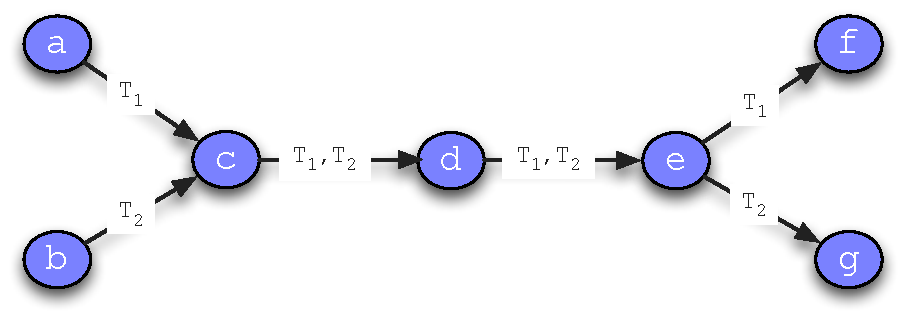
\includegraphics[scale=0.55]{figs/merger-example.pdf}
\caption{Example showing a subtree of two multicast trees, $T_1$ and $T_2$.  The edges used by each multicast tree are marked.}
\label{fig:merger-example}
\end{figure}


\subsubsection{Motivation: \basen Algorithm Inefficiencies}
\label{subsubsec:merge-motivate}

The \base multicast implementation creates a flow table entry at each node of a multicast tree that matches using the tree's multicast address. 
As a result, a switch, $v$, may have multiple flow table entries executing the same actions.  This occurs when multicast trees share the same outgoing links at $v$. 
\footnote{In cases where the tree can either be a primary tree or backup tree, we refer to the tree as a multicast tree.}
These inefficiencies are the motivation for developing the \merge algorithm, which replaces the set of flow table entries \base would create at $v$ with a single flow table entry. 
To do so, \merge writes a common identifier, or tag, in packet headers at the node immediately upstream from $v$. Using this tag, \merge creates a \emph{single} rule at $v$ to match and 
forward packets of \emph{all} trees with the same outgoing links at $v$.

Consider the simple example shown in Figure \ref{fig:merger-example} with two multicast trees $T_1$ and $T_2$. The directed links used by each tree are marked.
\base creates a flow table entry for $T_1$ at $a$, $c$, $d$, $e$, and $f$ and a flow table entry at $b$, $c$, $d$, $e$, and $g$ for $T_2$.  Because 
$T_1$ and $T_2$ both use the same outgoing links at $c$ and $d$, only a single forwarding rule is needed at each node.  This is what \merge creates and in the next two sections we describe how.

%In contrast, \merge leverages that $T_1$ and $T_2$ both use the same outgoing links at $c$ and $d$ to replace the two separate flow table entries at $c$ and $d$, created under \bases, with a single 
%forwarding rule. To do so, \merge first creates an action at $a$ and $b$ to write an identifier in the packet headers of all packets traversing $(a,c)$ and $(b,c)$.
%Then, at $c$ and $d$, \merge creates a single rule to match and forward packets based solely on this tag.




\subsubsection{\mergen Algorithm for Primary Trees}
\label{subsubsec:merge-primary}


\merge consolidates flow table entries at each node, $v$, where multiple primary trees share the same outgoing links. 
Upstream from $v$, \merge writes an identifier, or \emph{tag}, in packet headers and uses this tag to match packets at $v$ using a single rule shared by each of these primary trees.
%An identifier, or \emph{tag}, is used to match packets at $v$.  
%\merge writes this tag in the packet header at the node immediately upstream from $v$. % in the packet header of all packets corresponding to any of these multicast trees. 
The tag is removed downstream from $v$ where the trees diverge. 

A tag is a globally unique Ethernet address \merge writes in a packet header's {\tt dl\_dst} field (i.e., the Ethernet destination address).  When possible, \merge flow table entries use 
tags to match and forward packets, meaning that packets are matched solely on their {\tt dl\_dst} value.
When the same Ethernet address is applied to the packets of more than one multicast tree, we refer to this as a \emph{group tag}.  A \emph{single tag} is an 
Ethernet address used by only one tree. We use the term \emph{tag} to generically refer to either a group or single tag.
%\footnote{In some cases, packets corresponding to a multicast tree $T_i$ already have a tag written in their packet header upon reaching node $u$.  If this same tag is used to match packets 
%at $d$ where $(u,d) \in T_i$ no action is created at $u$ to write this same tag. However, for ease of explanation, we say that \merge writes the tag at $u$.}

\begin{figure}
  \centering
   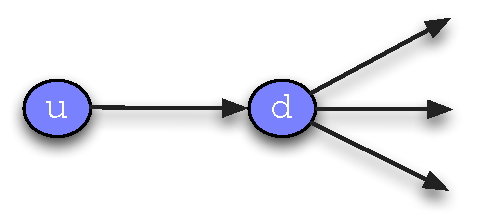
\includegraphics[scale=0.5]{figs/merger-ud.pdf}
\caption{Subgraph used to describe \merge in Section \ref{subsubsec:merge-primary}.}
\label{fig:merger-ud}
\end{figure}

%With these preliminaries in place, 
We are now ready to describe \merge in more detail.  
First, \merge marks the edges used by each primary tree.  Then, \merge executes a breadth first search of each primary tree, $T_i$, starting at its root.  
For each link $(u,d) \in T_i$ as shown in Figure \ref{fig:merger-ud}, \merge determines the match pattern to create at $d$ and the tagging actions to apply at $u$ using the following steps:
\footnote{Because $T_i$ is a tree, $(u,d)$ must be its only incoming link to $d$.  Therefore, we can determine $T_i$'s locally optimal tagging rule at $d$ by only considering $u$ and $d$.}
\begin{enumerate}

	\item Finds the set of trees, $S$, using $(u,d)$ that share the same outgoing links as $T_i$ at $d$. 

	\item If $|S| \geq 1$, \merge creates an action to write a group tag at $u$.  For each $T_j \in S \cup \{T_i\}$, \merge finds the rule at $u$ used to forward $T_j$ and appends an action
	to write a group tag to the rule's action list.
	Then, a single rule is created at $d$ that matches packets using this group tag and has an initial action list forwarding packets out the appropriate ports.

	\item If $S = \emptyset$, \merge peaks upstream at $u$ to determine whether to use a single tag or $T_i$'s multicast destination address to match $T_i$'s packets at $d$. 
	When $T_i$ is matched using either a single tag or its multicast destination address at $u$, \merge creates a rule at $d$ to match packets using a single tag and writes this single
	tag at $u$.  Otherwise, \merge creates a rule at $d$ matching packets using $T_i$'s multicast destination address (no action is needed at $u$).  
	%\footnote{If we were to write $T_i$'s single tag at $u$, this tag would be erroneously be applied to any other multicast tree using the same group tag as $T_i$ to match packets at $u$. }
	%Only when $T_i$ is matched using either a single tag or its multicast destination address at $u$, do we create a rule at $d$ to match packets using $T_i$'s single tag.  In which case, 
	%an action is created at $u$ to write this single tag.

\end{enumerate}
In step (3), we aim to use single tags to match packets because they allow \emph{any} backup tree to reuse $T_i$'s rule at $d$ by simply writing this tag at $u$.  
Whereas, if $T_i$'s multicast address is used to match packets at $d$, only $T_i$'s backup trees can reuse this forwarding rule (since $T_i$'s multicast address is unique to its multicast group).
We comment further on this design decision in the next section.

%In the Figure \ref{fig:merger-example} example, \merge leverages that $T_1$ and $T_2$ both use the same outgoing links at $c$ and $d$ to create a single rule at each node (as opposed
%to two separate flow table entries that would be created with \bases).  %After marking the edges used by $T_1$ and $T_2$, \merge
In the Figure \ref{fig:merger-example} example, \merge  creates an action at $a$ and $b$ to write a group tag in the packet headers of all packets traversing $(a,c)$ and $(b,c)$.
Then, at $c$ and $d$, \merge creates a single rule to match and forward packets based solely on this tag.  With regard to the breadth-first search (BFS) described earlier, 
\merge executes the following steps in  its breadth-first search (BFS) of $T_1$ at nodes $c$, $d$, and $e$.
%We describe the steps \merge executes in its breadth-first search (BFS) of $T_1$ at nodes $c$, $d$, and $e$.
At $c$, $S=\{T_2\}$ so \merge finds $T_1$'s rule at $a$ and includes an action to write a group tag, {\tt 12}, in all packets sent out $a$'s port to $c$. 
Then, \merge creates a flow table entry at $c$ that matches packets with {\tt dl\_dst = 12} and forwards packets out the port to $d$.  The same set of actions occur when the BFS reaches $d$. 
%except that no group tag needs to be written at $c$ because the same group tag
%At $e$, $S=\emptyset$ because $T_1$ and $T_2$ diverge. at $e$.  
\merge creates a forwarding rule at $e$ that matches packets using $T_1$'s multicast address and forwards these packets to $f$.



\subsubsection{\mergen Algorithm for Backup Trees}
\label{subsubsec:merge-backup}

Having discussed \merge for the primary tree case, we are now ready to extend \merge to generate forwarding rules for backup trees.  \merge 
aims to reuse forwarding rules of primary trees because these rules are already installed in the network, allowing the installation algorithm
(e.g., \pre or \posts) to avoid installation a new forwarding rule.  In cases where primary tree rules cannot be reused, \merge consolidates
flow table entries with other backup trees that have common forwarding behavior.

%We describe the case of generating forwarding rules for a set of backup trees, $\hat{T}^l$, using $l$. 
For a set of backup trees, $\hat{T}^l$, \merge generates backup tree forwarding rules as follows. 
\merge executes two rounds of BFS, traversing all
$\hat{T}^l_i \in \hat{T}^l$ in each round.  In the first round, for each $\hat{T}_i^l$, \merge finds each node where $\hat{T}_i^l$ has the same outgoing links as a primary tree.  
If so, $\hat{T}_i^l$ reuses the primary tree flow table entry at this node, $v$: \merge writes the primary tree tag at $v$'s parent node
allowing $\hat{T}_i^l$ packets to be forwarded using the primary tree rule, and makes no changes at $v$.

In the second round of BFSs, \merge consolidates flow table entries among the other backup trees for $l$
at nodes where primary tree tag reuse was not possible.  
To do so, the algorithm from Section \ref{subsubsec:merge-primary} is executed but comparing $\hat{T}_i^l$'s outgoing links with the outgoing links of 
each $\hat{T}_j^l \neq \hat{T}_i^l$ at nodes where $\hat{T}_i^l$ and $\hat{T}_j^l$ were unable to reuse primary tree tags. 

When \merge is applied to \pre and \post (referred to as \pres+\merge and \posts+\merges) the tag becomes the sole match criteria used by its flow table entry, with one exception.  This 
occurs with \pres+\merge when a {\tt bid} is required to distinguish between a backup and primary tree, as described in Section \ref{subsec:install-backups}. In those cases, the 
{\tt bid} and {\tt dl\_dst} fields are both used as match criteria.

%\merge attempts to reuse flow table entries of primary trees already installed in the network that share forwarding behavior with a backup tree. 
%First, \merge attempts to reuse flow table entries of primary trees already installed in the network that share forwarding behavior with a backup tree.  At nodes where this possible, no 
%flow table entry needs to be installed.  At the remaining nodes, % At nodes where this is not possible,
%\merge applies the procedure from Section \ref{subsubsec:merge-primary} to consolidate forwarding rules with other backup trees.  We detail these steps below. % for backup trees of link $l$.



%Under \merge we can avoid matching using a tree-id at any $d \in D^l_i$ where $\hat{T}_i^l$ uses a group tag or reuses a primary tree tag. 
%These tags are applied upstream from $d$ and are different from any tags $T_i^l$ uses  a $d$.  The tree-id is only required at $d \in D^l_i$ where \merge is forced to 
%match $\hat{T}_i^l$'s multicast address or single tag.  \merge described in Section \ref{subsec:merge-backup}, is modified to incorporate this additional match criteria. 

\subsubsection{\mergen Discussion}
\label{subsubsec:merge-discuss}

%Now that we have presented the core of aspects of \merges, we comment on. We comment on a number of 
To unify our presentation of \merges, we comment on some of the properties of the algorithm along with the implications of using \merge on other important aspects of \mdrs.
%In the following order, we discuss the advantages of using \merges, \merge time complexity, \merges's implications on garbage collection, \merges's ``do not harm'' property, and
%how \pcnt monitors \merge flows. 

{\bf Benefits.}
In comparison with \bases, \merge reduces the number of forwarding rules required to install each multicast tree.  As a result,
\merge is more space efficient and can yield faster backup tree installation.
%By reducing the number of forwarding rules required to install each multicast tree, \merge is more space efficient and can yield faster backup tree installationi with \posts+\merges.
Recall that for each primary tree, \mdr pre-computes a backup tree for each of its links.  In this scenario \pres+\merge can significantly reduce the number of pre-installed rules.
These savings are especially important because, as noted in Section \ref{subsec:openflow}, OpenFlow switches can only support a limited number of flow table entries.
With \posts, \merge can yield faster recovery because fewer backup tree flow table entries translates into fewer control messages to activate backup trees.

{\bf Time Complexity.}
Like \bases, \merge complexity is bounded by the breadth-first search (BFS) executed for each of the $m$ multicast trees given as input.  At each node, $v$, visited in the BFS, \merge
compares the out-links used by all other multicast trees that use $v$.  Since there can be at most $m$ such trees, this takes $O(m)$ time.  If we let $n$ be the number of graph nodes,
each BFS takes $O(mn)$ time \footnote{BFS has $O(|V|+|E|)$ complexity. In our case, each BFS is over a directed tree, meaning the number of edges traversed in each BFS is $O(n-1)$.  
Therefore, we can simplify BFS time complexity to $O(n)$.}
and the total time complexity of \merge is $O(m^2n)$.

% O( V+E), is O(V) because we are dealing with trees
% each BFS step has O(m) complexity, since need to check the out-links of all other trees using v
%  m x O(mn) -- O(m^2n)

{\bf Garbage Collection}.
\mdrs's garbage collection algorithm remains unchanged from the description in Section \ref{subsec:garbage}.  
Recall that {\tt rule\_map} is a dictionary that maps the flow table entry installed at each node to the
set of backup and primary trees using the flow table entry. The only difference between \base and \merge garbage collection is the number of stale rules it identifies (likely fewer
stale rules with \merges) not how the stale rules are found.  
As with \bases, \merge garbage collection can find any stale forwarding rules by consulting {\tt rule\_map}.


%Garbage collection
%Under our \base multicast implementation, garbage collection is straightforward.  The controller maintains a dictionary, {\tt rule\_map}, for each node, mapping
%each multicast tree (primary tree and backup trees) using $v$ to the flow table entry installed at $v$. When a link, $l$, fails the garbage collection routine determines 
%the set of stale forwarding rules for each $T^l_i$. A stale rule exists at each $v \in V_i \setminus \hat{V}_i^l$ (i.e., nodes unique to the primary tree) and each $d \in D_i^l$ 
%(nodes where the backup tree diverges from the primary tree).  The controller consults {\tt rule\_map} to find the forwarding rule at each node and either sends an explicit 
%remove flow message to each of these nodes (if using a hard state signaling scheme \cite{HardSoftState}) or allows the forwarding rule to time out (with a soft state algorithm \cite{HardSoftState}).

%With \merges, garbage collection adds an additional check before removing any candidate stale flow table entry, $c_v$, found using the procedure described in the previous paragraph.  
%Garbage collection consults {\tt rule\_map} to determine if any other primary tree or newly installed backup tree uses $c_v$, if so 
%is modified to check that no other primary tree 

%\merge complicates garbage collection because it is no longer the case that an installed flow table entry is used by a single multicast tree (e.g., multiple primary trees
%can share the same flow table entry).  Garbage collection must now consider that a different set of primary trees
%use flow table entry, $e$, before $l$ fails versus after $l$ fails and backup trees $\hat{T}^l$ are installed.  To account for this, we modify the first step of garbage collection.  
%Rather than simply add $T_i$'s flow table entry, $e_v$, at each $v$ to $E_r$, the garbage collection first checks if any newly installed tree (i.e., each tree in $\hat{T}^l$) reuses $e_v$. Then, we
%check if any primary tree unaffected by $l$ failing (i.e., each tree in $\bar{T}^l$) uses $e_v$. If either of these checks is positive, $e_v$ is 
%not included in $E_r$ but {\tt flow\_map} is updated for $T_i$.  Otherwise, $e_r$ is added to $E_r$ and {\tt flow\_map} is updated for $T_i$.

%\item \underline{Garbage Collection}: keep track of flows used by each tree.  garbage collection ensures flows of unaffected trees are not removed.

{\bf Do No Harm.} 
We say that \merge is an algorithm that does ``no harm''  \footnote{This is similar in spirit to the Hippocratic Oath taken by physicians that they will ``never do harm [to patients]'' }
because (a) \merge never creates more flow table entries than \base and (b) when generating rules for backup trees, \merge makes no modifications to flow table entries of primary trees that do not use the 
failed link. We informally prove each of these properties below.

Regarding (a), consider an arbitrary multicast tree (primary of backup tree), $T_i$. \merge creates at most one flow table entry at any $v \in T_i$.  
The flow table entry, $e_i$, either matches and forwards packets using a group tag, a single tag, or using the $T_i$'s multicast address.  Any $e_i$ tagging actions 
are simply appended to $e_i$'s action list (when \merge visits $T_i$'s children of $v$), requiring the creation of no additional flow table entries.  We conclude that in the worst case,
\merge creates the same number of flow table entries as \bases.  

Now consider property (b) where we let $T_j$ refer to a primary tree not using $l$. By construction, \merge only creates flow table entries and new actions for the backup trees of 
link $l$ (i.e., $\hat{T}^l$). These flow table entries have distinct match criteria than those \merge creates for $T_j$.  If a backup tree reuses $T_j$'s flow table entry at $v$, 
no changes are made to this flow table entry.  Lastly, \mdrs's garbage collection algorithm ensures that no $T_j$ flow table entry is removed.

%As an aside, \merges's do no harm property ensures that under \merges, garbage collection has fewer flow table entries to remove than with \bases.  Intuitively, this 
%is reasonable because \merge seeks to reuse primary tree flow table entries. 


{\bf Optimality}.  
Because \merge makes tagging decisions locally at each node, $v$, based only on the multicast trees using $v$'s outgoing links and the tags used at $v$'s parent nodes,
\merge does not always yield the minimum set of forwarding rules.
Consider again Figure \ref{fig:merger-example} but replace $T_1$ with $S_1$ and $T_2$ with $S_2$, where $S_1$ and $S_2$ are sets of multicast trees of size $k$.
%$S_1=\{T_1,T_2,...,T_k\}$ and $S_2 = \{T_{k+1},T_{k+2},...,T_{2k+1}\}$.  
In this scenario, \merge writes the same group tag, denoted {\tt 12}, at $a$ and $b$ for each tree in $S_1$ and $S_2$.  Then, at $c$ and $d$ \merge installs a single rule that matches and forwards 
using the {\tt 12} tag.  Lastly, for each $T_i \in S_1 \cup S_2$, a rule is created at $e$ that matches packets using each $T_i$'s multicast address.  %This results in 

A better solution in this example is to use a different group tag for $S_1$ and $S_2$.  Under this proposal, let {\tt 11} be the group tag applied to each tree in $S_1$ 
at $a$ and {\tt 22} the tag we write 
in the packet header of each tree in $S_2$.  These group tags can be used create two separate rules at $c$, $d$, and $e$ to forward $S_1$ packets based on {\tt 11} and $S_2$ packets using {\tt 22}.
By using different tags for $S_1$ and $S_2$, we avoid having to create $2k$ separate rules for each tree in $S_1 \cup S_2$ at $e$, clearly a better solution that the 
one produced by \merges. 

This example suggests that an algorithm, $\mathcal{A}$, that finds the minimum number of forwarding rules for a set of multicast trees $T$ 
must consider, for $S \subseteq T$ where each multicast tree $S_i \in S$ uses link $(u,d)$, how each of $S$'s subsets share links downstream from $d$.
Since this requires computing the power set of $S$ and there are an exponential number of ways $S$'s subsets can use common links downstream from $d$,
we conjecture that no polynomial time $\mathcal{A}$ exists. %a polynomial time algorithm that yields the optimal  solution does not exist.





%The single group tag used at u forces a separate rule to be created for each tree in S if not all S have the same outports at d.  In some cases, it is beneficial to partition S into subsets, 
%based on links shared downstream, and use a group tag unique to each subset to match and forward packets downstream. 

%Consider the following example.  S_1 and S_2 denote a set of trees and let S = S_1 \cup S_2.   Merger creates an action at a and b to write group tag, denoted 12,  for each tree in S_1 and S_2.  Then, at u a single rule matches and forwards using the 12 tag.  Lastly, a rule is created at d for each tree in S that matches using the tree's destination address to ensure correct forwarding at d.  A better approach is to write group tag 11 at a for S_1 and group tag 22 for S_2 at b.   We can use these group tags to match and forward -- using two separate rules -- at u and d using group tags 11 and 22.   Using different tags for S_1 and S_2 makes it unnecessary to create a separate rule for each tree in S at d.   The same challenge arises if u and d were connected using additional links all used by S. 

{\bf Implications for \pcnts.}
\pcnt requires no changes to monitor packet loss of flows forwarded using \merge rules. However, we make 
the case here that \merge can improve the accuracy of \pcnt loss rate estimates and reduce the time to compute these estimates.  In Section
\ref{subsec:eval-pcount}, we will find that our simulations bear out the qualitative argument made here.

% (a) can tune k.  cost associated with each k
Recall from Section \ref{subsec:pcnt} that with \pcnt the number of monitored flows, $k$, can be tuned.
Determining an appropriate $k$ parameter involves a trade-off between the accuracy of packet loss estimates and time: larger $k$ yield more accurate packet loss estimates
but at the cost of slower detection times (the time between when packet loss occurs and when it is detected). Detection times of a monitored link, $(u,d)$, increase with larger $k$
for two reasons. One, for each of the $k$ flows, \pcnt makes a copy of the flow's forwarding rule at $u$ and $d$ in order tag and count packets.  Two, 
\pcnt sends $k$ queries to $u$ to read the state of each flow table entry generated by \pcnts. % generated flow table entry and a single aggregate statistic query to $d$.

%a function of the number of statistic queries \pcnt sends. % to the switches of a monitored link.  
%Recall from Section \ref{subsec:pcnt}, when estimating packet loss of a link, $(u,d)$, \pcnt makes a copy of the flow table entry at $u$ and $d$, for each flow \pcnt monitors. 

With \merge the same flow table entry, $e_i$, can be used by multiple ($r$) flows.  In these cases, \pcnt only needs to explicitly monitor one of these flows to measure
the packet loss of all $r$ flows.  That is, \pcnt can monitor the loss of all $r$ flows with cost of monitoring a single flow:
the one copy of $e_i$ \pcnt makes at $u$ and $d$ ensures that packets of any of these $r$ flows are tagged and counted and
only a single statistic query is needed to retrieve $e_i$'s packet count.

Consider the example in Figure \ref{fig:intuition-example-t1} and suppose that \pcnt monitors link $(g,l)$. 
Two multicast flows -- $f_b$ for primary tree $T_b$ and $f_c$ for primary tree $T_c$ -- traverse
$(g,l)$.  \base creates a separate forwarding rule for $f_b$ and $f_c$ at $g$ while \merge generates a single forwarding rule at $g$ used by both $f_b$ and $f_c$.  As a result, 
with \merges, \pcnt can track the  packet loss of $f_b$ and $f_c$ by querying just the shared \merge forwarding rule at $g$ (rather than interact with two separate \base forwarding rules).
These savings are quantified using simulations in Section \ref{subsec:eval-pcount}.

%Recall from Section \ref{subsec:pcnt} that with \pcnt the number of monitored flows, $k$, can be tuned.  Determining an appropriate $k$ parameter involves a trade-off between the accuracy of
%packet loss estimates and time: larger $k$ yield more accurate packet loss estimates but at the cost of slower detection times (the time between when packet loss occurs and when it is detected).
%Detection times of a monitored link, $(u,d)$, are a function of the number of statistic queries \pcnt sends. % to the switches of a monitored link.  
%\pcnt sends a read state query for each monitored flow to $d$ and a single statistic query to $d$.

%As a mechanism to count packet loss, \pcnt makes a copy of the flow table entry of each monitored flow where the flow table entry copy upstream tags packets upstream and a second flow table entry copy counts 
%tagged packets downstream.  Because with \merge the same flow table entry, $e_i$, may be shared by multiple flows, all of these flows can be monitored at the cost of monitoring a single flow: 
%only a single \pcnt statistic query is needed to retrieve $e_i$'s packet count rather than one separate query per flow using $e_i$ that would necessary with \bases.  






\section{Related Work}
\label{sec:related-pmu}

\full is well-studied \cite{Baldwin93,Brueni05,Haynes02, Mili90, Xu04}.  
Haynes et al. \cite{Haynes02} and Brueni and Heath \cite{Brueni05} both prove \full is NPC.  
However, their proofs make the unrealistic assumption that all nodes are zero-injection.  We drop this assumption and thereby generalize their NPC results for \fulls.
Additionally, we leverage the proof technique from Brueni and Heath \cite{Brueni05} in all four of our NPC proofs, although our proofs
differ considerably in their details. 

%The power systems literature generally ignores the fact that PMUP is NP-Complete because, in practice, power system graphs are small enough to allow for an exact solution to be found.
In the power systems literature, Xu and Abur \cite{Xu04,Xu05} use integer programming to solve \fulls, while Baldwin et al. \cite{Baldwin93} and Mili et al. \cite{Mili90} use simulated annealing 
to solve the same problem. All of these works allow nodes to be either zero-injection or non-zero-injection.  However,
these papers make no mention that \full is NPC, i.e., they do not characterize the fundamental complexity of the problem. 
%The work of Xu and Abur \cite{Xu04} and Phadke et al. are representive of the power systems approach to the problem: formulate the problem as integer 
%program and use an integer programming solver to find the optimal PMU placement.  

Aazami and Stilp \cite{Aazami07} investigate approximation algorithms for \fulls.  They derive a hardness approximation threshold of $2^{\log^{1 -\epsilon}n}$.
Also they prove that in the worst case, {\tt greedy} from Section \ref{sec:approx} does no better $\Theta(n)$ of the optimal solution.  However, this approximation ratio assumes that 
all nodes are zero-injection.
%We leverage this approximation result in proving the approximation ratios of our heuristic-based algorithms.

Chen and Abur \cite{Abur06} and Vanfretti et al. \cite{Vanfretti10} both study the problem of bad PMU data. Chen and Abur \cite{Abur06} formulate their problem differently than \xval and \xvalparts.  
They consider fully observed graphs and add PMUs to the system to make all existing PMU measurements non-critical 
(a critical measurement is one in which the removal of a PMU makes the system
no longer fully observable). Vanfretti et al. \cite{Vanfretti10} define the cross-validation rules used in this paper.  They also derive a
lower bound on the number of PMUs needed to ensure all PMUs are cross-validated and the system is fully observable. 



\section{Evaluation}
\label{sec:evaluation}

We implement each algorithm from Section \ref{sec:algs} in the POX OpenFlow controller \cite{Pox} and run simulations using the Mininet 2.0.0 virtualization 
environment \cite{Lantz10}.  Simulations run on a Linux machine 
with four 2.33GHz Intel(R) Xeon(R) CPUs and 15GB of RAM.  Mininet is configured to run inside Oracle's VirtualBox \footnote{\url{https://www.virtualbox.org/}}
virtual machine and is allocated 4GB RAM and a single CPU.  
All generated virtual networks use Mininet's default software switch, Open vSwitch \footnote{\url{http://openvswitch.org/}}.  Unless otherwise noted, the \mdr 
controller algorithm runs inside the VirtualBox VM.


% Open vSwitch -- software switch, POX (OpenFlow controller), 

\subsection{Link Failure Detection Simulations}
\label{subsec:eval-pcount}

We run two sets of Mininet-based simulations to evaluate \pcnts. First, we measure the accuracy of \pcnt loss probability estimates and quantify how accuracy improves as more flows are monitored. 
Then, we consider how controller and switch processing time increases as \pcnt monitors more flows. 
%Unfortunately, switch processing time results are skewed because Mininet's software switch, Open vSwitch, 
%does not offer performance fidelity \cite{Lantz10}.  We comment further on this issue later in this section. 

%study the tradeoff between improving the accuracy of \pcnt packet loss estimates by monitoring more flows and the resulting increase in switch processing time 
%First, we study how the number of flows \pcnt monitors affects the accuracy of its packet loss estimates. Then, detection time is quantified as a function of the number of monitored flows.  
%Our simulations configure \pcnt such that all measurement windows are non-overlapping.  
%This means that for each window, $w$, \pcnt accounts for every dropped packet of a monitored flow, 
%meaning that the accuracy of \pcnt loss estimates are determined by its window size ($w$) and the number of monitored link flows ($k$).

%We can modify \pcnts's window size ($w$) and number of monitored link flows ($k$) to control the number of packets \pcnt uses to estimate the loss rate.  
%In this simulation, we evaluate 
%hus, the accuracy of \pcnt loss rate estimates are a function of the number of packets considered in a sampling window $w$. 

%{\bf Setup.}
{\bf Accuracy of Loss Probability Estimates.}
For the dumbbell topology shown in Figure \ref{fig:eval-pcount-setup}, we use \pcnt to measure the packet loss over link $(u,d)$.  We generate $m$ multicast groups
where each $h_1,h_2, ..., h_m$ multicasts packets to terminal nodes $s_1, s_2, ..., s_m$ at a constant rate of $60$ packets per second, the standard sampling rate of PMUs.  \base is used
to implement multicast, resulting in $m$ separate flow table entries at $u$ and $d$.  At the end of the section we comment how our results apply to \merges. We let $m=\{10,20,30,40,50\}$
\footnote{Simulations run prohibitively slow for $m>50$ due to CPU overload.} %the CPU overhead of each of the $m$ constant bit rate flows made each simulation run prohibitively slow.}
and, using Mininet, drop packet traversing $(u,d)$ using a Bernoulli process with loss probability $p=\{.01,.05,.10\}$.  
%Let $w$ be \pcnt loss estimates are a function of its window size ($w$) and number of monitored link flows ($k$).

%In this simulation, we measure how close \pcnt loss probability estimates are to $p$ for different $w$ and number of monitored flows ($k$).
In this simulation, we quantify how the accuracy of \pcnt loss estimates -- measured relative to the true underlying loss rate, $p$ -- as we modify the number of flows \pcnt monitors. 
Recall from Section \ref{subsec:pcnt} that \pcnt accounts for every dropped packet of a flow it monitors, meaning that the only error in \pcnt estimates results from unmonitored flows.
%Here we quantify how the accuracy of \pcnt loss estimates change as we modify the number of flows \pcnt monitors.  
Because the same trends hold across all $m$ and $p$ values, we describe a single representative case, where $m=10$ and $p=.05$, below.
%We find the same trends hold across all $m$ and $p$ values.  A representative case, where $m=10$ and $p=.05$, is described below.

%This means that for each window, $w$, \pcnt accounts for every dropped packet of a monitored flow, 
%meaning that the accuracy of \pcnt loss estimates are determined by its window size ($w$) and the number of monitored link flows ($k$).

Figure \ref{fig:pcount-loss-windows} compares the $95\%$ confidence intervals of \pcnts's link loss probability estimates -- centered around the true loss probability ($.05$) for consistency -- 
as a function of window size $w =\{0.5,1,...,5\}$ seconds. \pcnt is configured such that each measurement window starts only after the packet loss from the previous window has been computed.
Results are shown where \pcnt monitors $k=\{10\%,40\%,70\%,100\%\}$ of $(u,d)$ flows (each monitored flow is selected randomly).  The confidence intervals for each $w,k$ pair are computed
over $100$ simulation runs.

% in which each monitored flow is selected randomly. 
%For consistency, the $95\%$ confidence interval curves are centered around the true loss probability ($.05$). 

\pcnt loss rate estimates are extremely accurate: the $95\%$ confidence interval, across all $w$ and $k$, lies within $15\%$ of the true loss probability.  This is the case even when \pcnts's 
estimate is based on only $30$ packets (occurs when $k=10\%$ and $w=0.5$).  Figure \ref{fig:pcount-loss-pkts}, which plots link loss probability estimates as a function of the number of 
packets considered during each simulation run, shows that after \pcnt considers $75$ packets its mean loss probability estimate is within $2\%$ of the true loss probability.  
\footnote{This accuracy is not surprising since loss probability estimate is averaged over $100$ simulation runs.}
As expected, \pcnt accuracy increases with larger $k$.  For each $k$, the standard deviation (of \pcnt loss probability estimates) decreases as a function of the square root of $w$.  
%However, since \pcnt loss rate estimates are 

%Figure \ref{fig:pcount-loss-pkts} plots link loss probability estimates as a function of the number of packets considered during each simulation run.  
%After \pcnt considers $75$ packets its mean loss probability estimate is within $2\%$ of the true loss probability.  This accuracy is not surprising since loss probability estimate is 
%averaged over $100$ simulation runs. 


%Since \pcnts's aim is to estimate loss probabilities over a single window, a more telling statistic is the standard deviation. Figure \ref{fig:pcount-loss-windows} 
%shows that the standard deviation, for each $k$, decreases as a function of the square root of $w$.  The same trend holds when we %consolidate the four curves from Figure \ref{fig:pcount-loss-windows}
%plot the same link loss probability estimates as a function of the number of packets, rather than window size, \pcnt considers over each simulation run (Figure \ref{fig:pcount-loss-pkts}).
%We find that after \pcnt considers approximately $750$ packets, the confidence intervals lie within $20\%$ of the true probabilities, suggesting that individual \pcnt loss probability
%estimates are extremely accurate.   %Accuracte loss estimates were expected because 


{\bf Processing Time.}
%Next we quantify the processing time at the network switches in handling \pcnt statistic queries. [mention this is the primary time] 
%Next, we quantify switch processing time associated with handling \pcnt statistic queries. 
Next, we quantify how \pcnt processing time increases when \pcnt monitors additional flows.  We measures packet loss over $(u,d)$ from Figure \ref{fig:eval-pcount-setup}.
Processing time is measured as the time between when \pcnt sends its first statistic query and when \pcnt computes its packet loss estimate. Recall from Section \ref{subsec:pcnt} 
that if \pcnt monitors packet loss of $k$ flows traversing $(u,d)$, \pcnt sends $k$ statistic queries to $u$ and one aggregate query to $d$. 

\pcnt is configured such that each measurement window starts only after the packet loss from the previous window has been computed. Additionally, \pcnt window size is fixed to $2$ and 
the loss threshold is set to $0$.
Because Mininet multiplexes CPU resources using the default Linux scheduler, we found that running the constant rate PMU flows introduces unwanted CPU contention, adding noise to 
our results.  For this reason, we create only a single multicast group (with source $h_1$ and a single sink $s_1$) 
but do not actually send any packets between the two hosts. To further reduce CPU contention, we run \pcnt as a remote control application, outside of the VirtualBox VM.

As computed, processing time accounts for (a) the time at the controller
to generate $k+1$ statistic queries, (b) the transmission delay associated with sending the $k+1$ statistic queries from the controller to $u$ and $d$, 
(c) the network delay in sending each statistic query from the controller to switch, (d) total time to process the statistic query at $u$ and $d$, (e) the delay in sending the $k+1$ query results
from switch to controller, and (f) the latency in receiving and recording statistic query replies at the controller. % and computing packet loss at the controller. 
We subtract (c) and (e), the network delay between controller and switches, from the measured processing times.  Because the combined delay of (a), (b), and (f) accounts for less
than $1\%$ of the overall processing time, part (d), the time to process statistic queries at $u$ and $d$, determines the overall processing times.



%Recall from Section \ref{subsec:pcnt} that if \pcnt monitors packet loss of $k$ flows traversing $(u,d)$, \pcnt sends $k$ statistic queries to $u$ and one aggregate query to $d$. 
%We measure detection time as the time between when \pcnt sends its first statistic query and when \pcnt computes its packet loss estimate.  This time window accounts for (a) the time at the controller
%to generate $k+1$ statistic queries, (b) the transmission delay associated with sending the $k+1$ statistic queries from the controller to $u$ and $d$, 
%(c) the network delay for each statistic query to reach the appropriate switch, (d) total time to process the statistic query at $u$ and $d$, (e) the delay in send the $k+1$ query results
%from switch to controller, and (f) the latency in receiving and recording statistic query replies. % and computing packet loss at the controller. 

%\footnote{We did additionally measure the time to generate and send OpenFlow statistic queries from the controller, along with time to process and record query results at the controller. 
%This controller processing time is insignificant when compared to switch processing time: at most total controller processing time is $150$ times smaller than the total switch processing time. }
%Using the topology from Figure \ref{fig:eval-pcount-setup}, we monitor packet loss over $(u,d)$. \pcnt is configured such that each measurement window starts only after the packet loss from
%the previous window has been computed. Additionally, \pcnt window size is fixed to $2$.  

%Recall from Section \ref{subsec:pcnt} that if \pcnt monitors packet loss of $k$ flows traversing $(u,d)$, \pcnt sends $k$ statistic queries to $u$ and one aggregate query to $d$.  
%We measure the total switch processing time as the time between when \pcnt sends its first and last statistic query, minus the average controller-to-switch delay.  

Figure \ref{fig:pcount-dtime} shows the processing time, computed as described in the previous paragraph, as a function of the number of flows \pcnt monitors, $k$.
\footnote{Fake multicast groups and corresponding flow table entries are generated and installed at $u$ and $d$ in cases where \pcnt monitors more than the $1$ multicast group.}
Each data point is the mean computed over $50$ simulation runs. To measure the effect of flow table size on query processing time, we install $r$ additional flow table entries at $u$ and $d$.

We find that processing time increases quadratically with $k$ and there is a significant gap in processing time between each $r$.  In practice, we expect non-empty flow tables so the $r=0$ curve
is overly optimistic.  Therefore, to reasonably achieve sub-second processing time, our results show that fewer than $75$ flows can be monitored. 

Because the switches are completely idle during each simulation run, except for the time to process the read state queries, and the software switches used have
considerably more powerful CPUs relative to hardware switches \cite{Curtis11,Rotsos12}, these results likely underestimate processing time.  
Nonetheless, these results underscore the high cost in monitoring a large number of flows. 
%We expect the query processing 

%Due to Mininet's lack of performance fidelity, each statistic query takes $O(r+k)$ time to process rather than $O(1)$ time (provided by real hardware switches) \cite{Lantz10}. As a result,
%processing time increases quadratically with $k$ and there is a significant gap in processing time between each $r$.  If real hardware switches were used, we would expect
%processing time to increase linearly as $k$ grows and that the four separate $r$ curves from Figure \ref{fig:pcount-dtime} would collapse into one single curve.

{\bf Summary.}
%Although the processing time results are skewed in favor of \pcnts, the slow processing times associated with monitoring large numbers of flows and the highly accurate loss estimates
The slow processing times associated with monitoring large numbers of flows and the highly accurate loss estimates for even small $k$ strongly suggest that $k$ should be small.
Because the software switch skews the processing time results in favor of \pcnts, we expect that even a stronger case for using small $k$ can be made using hardware switches.
However, we caution that the (Bernoulli) loss process is biased in favor of \pcnt because we found loss rates to be nearly uniform across all flows traversing $(u,d)$.

%that a trade-off between accuracy and processing time exists when determining
%negatively by a factor of $r+k$, the results underscore that a trade-off between accuracy and processing time exists when determining
%how many flows to monitor with \pcnts. Fortunately, we found \pcnt loss estimates to be highly accurate even when monitoring a small percentage of flows ($10\%$) traversing $(u,d)$, suggesting
%that small $k$ should suffice.  As further evidence, we observed a small marginal increase in accuracy along with a significant penalty (in terms of detection time) resulting from using 
%large $k$.  However, we caution that the (Bernoulli) loss process is biased in favor of \pcnt because we found loss rates to be nearly uniform across all flows traversing $(u,d)$.

%In Section \ref{subsec:merge}, we stated that \merge can speed \pcnt processing because, with \merges, \pcnt can install and query fewer flow table entries to achieve similar accuracy results
%when monitoring more \base flows.
%reduce switch processing time by reducing the number of \pcnt statistic queries since multiple flows may be using the same forwarding rule. 
%Our results suggest that the savings in processing time can be significant. 

%The trade-off between accruacy and processing time suggests that \merge can improve \pcnt results.  As detailed in Section \ref{subsec:merge}, \merge can reduce the 

%In summary, determining how many flows to monitor involves a trade-off between accuracy and processing time.Although processing times from our simulations are skewed negatively by a factor of $r+k$, the results underscore the significant penalty (in terms of detection time) in monitoring a large number of flows. 
%Fortunately, we find \pcnt loss estimates to be highly accurate even when monitoring a small percentage of flows ($10\%$) traversing $(u,d)$.  This allows for fast and accurate packet loss detection.%Further, the impressive accuracy of \pcnt results when monitoring a small percentage ($10\%$) of flows suggest that only a fraction of flows need to be monitored. 

%Our findings also confirm that our conjecture in Section \ref{subsec:merge} that \merge can improve \pcnt results.  Recall that \merge replaces individual forwarding rules (when possible) that 
%have the same set of
%outports with a single flow table entry. As a result, when \pcnt copies the flow table entry, $e_i$, of a monitored flow, $f_i$, for tagging and counting purposes, \pcnt indirectly monitors all other 
%flows using $e_i$ (as a result of \merges).  This allows \pcnt to derive the accuracy gains of monitoring multiple flows (each flow using $e_i$) but at the cost of monitoring a single flow 
%(only a single \pcnt statistic query must be sent to $u$, rather than one query per flow using $e_i$). 
%to estimate loss over a sample of more than $60$ packets/second, thereby boosting accuracy, yet only a single \pcnt statistic query must be sent to $u$ (rather than one query per flow using $e_i$

%when \pcnt monitors a flow, $f_i$, $f_i$ may map to a rule, $e_i$, used by multiple flows.  By tagging and counting all packets matching $e_i$, \pcnt estimates loss over a sample
%of more than $60$ packets/second, thereby boosting accuracy, yet only a single \pcnt statistic query must be sent to $u$ (rather than one query per flow using $e_i$).

%{\it [TODO]: mention \merge is beneficial because fewer queries.  this is the case whether query processing time is linear or constant}
%
%{\it [TODO]: In summary, determining how many flows to monitor involves a trade-off between accuracy and processing time.  Although processing times are skewed by a factor of $r+k$, 
%the results underscore the significant time penalty (in terms of detection time) in monitoring a large number of flows.  Further, the impressive accuracy of \pcnt results even when 
%a small percentage ($10\%$) of flows are monitored suggest that only a fraction of flows need to be monitored. } 


%\begin{figure*}[t]
%  \begin{center}
%  	\subfigure[Dumbbell topology used in the \pcnt evaluation.]{ \label{fig:pcount-res}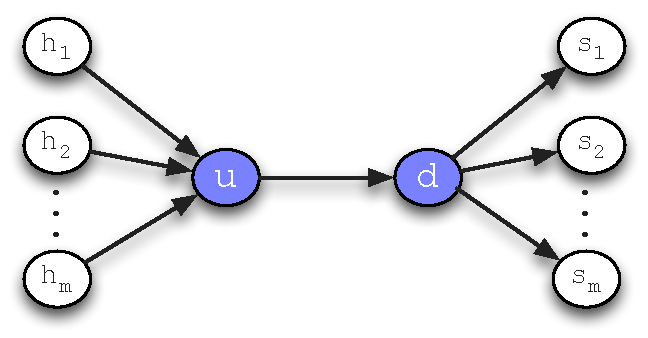
\includegraphics[scale=0.51]{figs/pcount-setup.pdf}}
%    \subfigure[Loss estimates as function of \pcnt window size.]{\label{fig:pcount-loss-windows}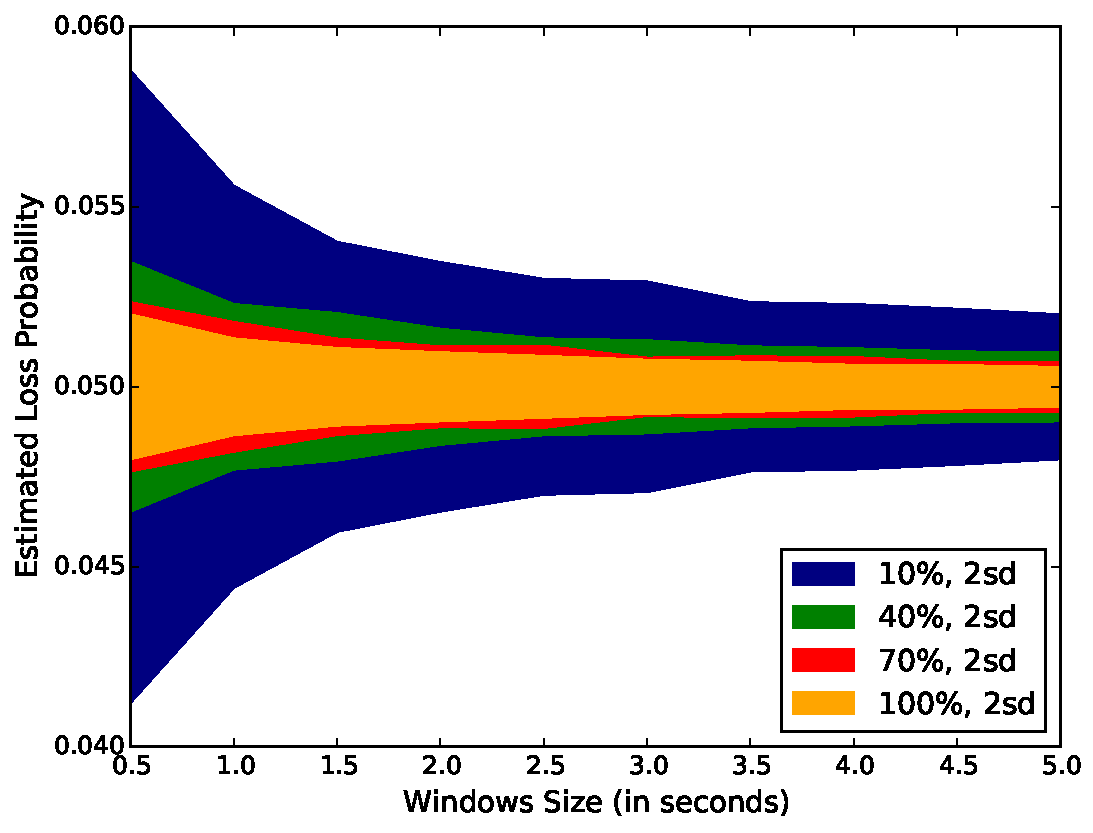
\includegraphics[scale=.33]{figs/pcount-loss-windows.pdf}}
%    \subfigure[Loss estimates as function of number of packets.]{\label{fig:pcount-loss-pkts}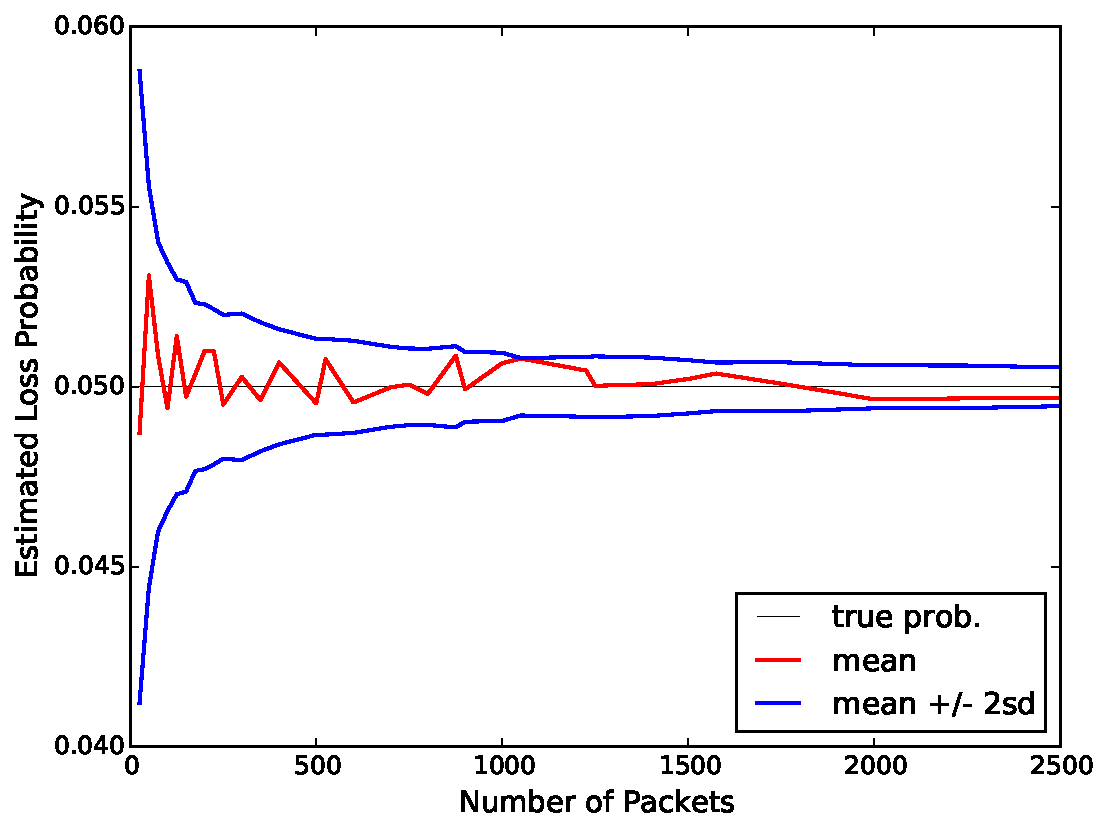
\includegraphics[scale=0.33]{figs/pcount-loss-pkts.pdf}}
%  \end{center}
%	\caption{Accuracy of \pcnt loss probability estimates over a single link, $(u,d)$, from Figure \ref{fig:eval:pcount-setup}.}
%  \label{fig:pcount-res}
%\end{figure*}


\begin{figure}
  \centering
   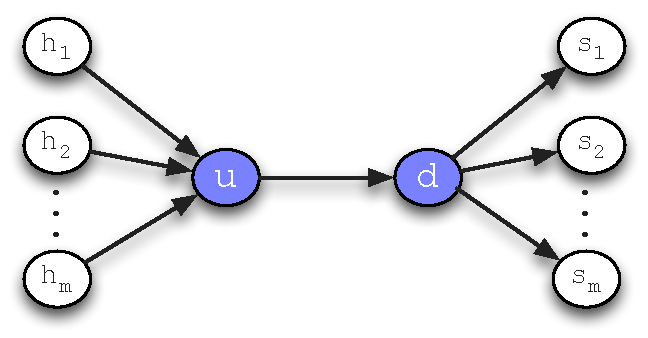
\includegraphics[scale=0.75]{figs/pcount-setup.pdf}
\caption{Dumbbell topology used in the \pcnt evaluation.}
\label{fig:eval-pcount-setup}
\end{figure}

\begin{figure*}[t]
  \begin{center}
    \subfigure[Loss estimates as function of \pcnt window size.]{\label{fig:pcount-loss-windows}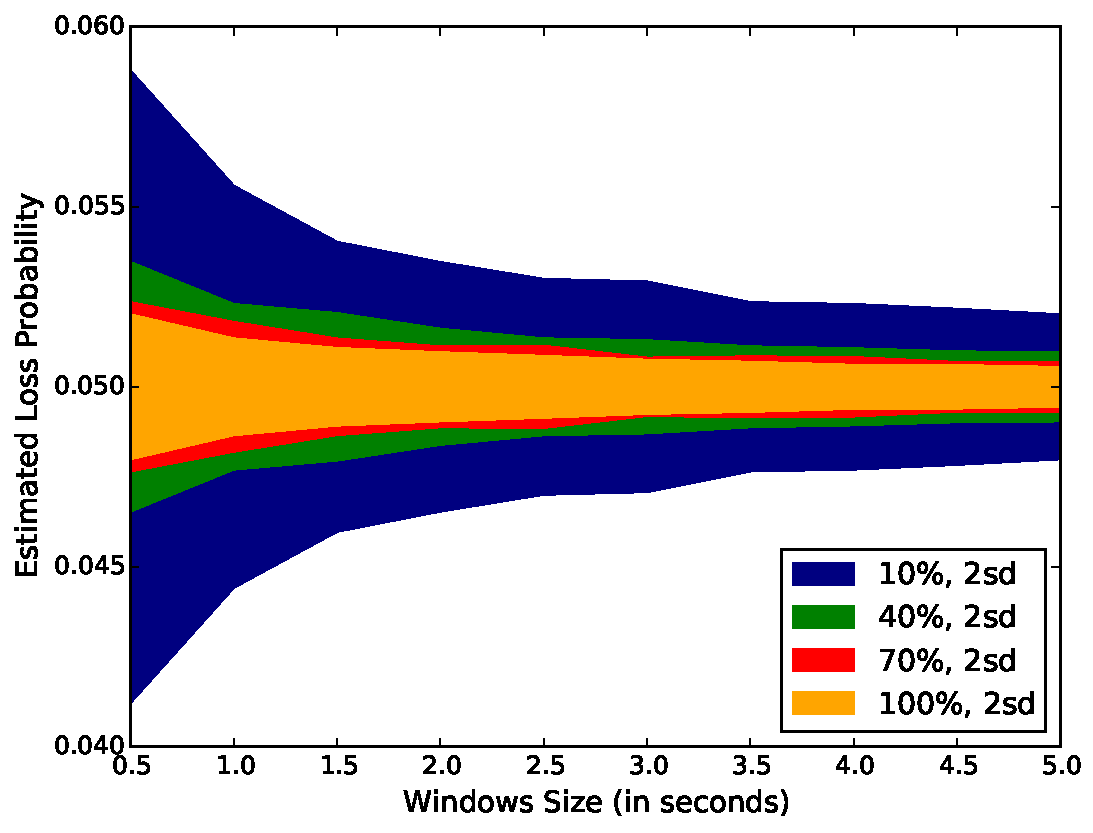
\includegraphics[scale=0.4]{figs/pcount-loss-windows.pdf}}
    \subfigure[Loss estimates as function of number of packets.]{\label{fig:pcount-loss-pkts}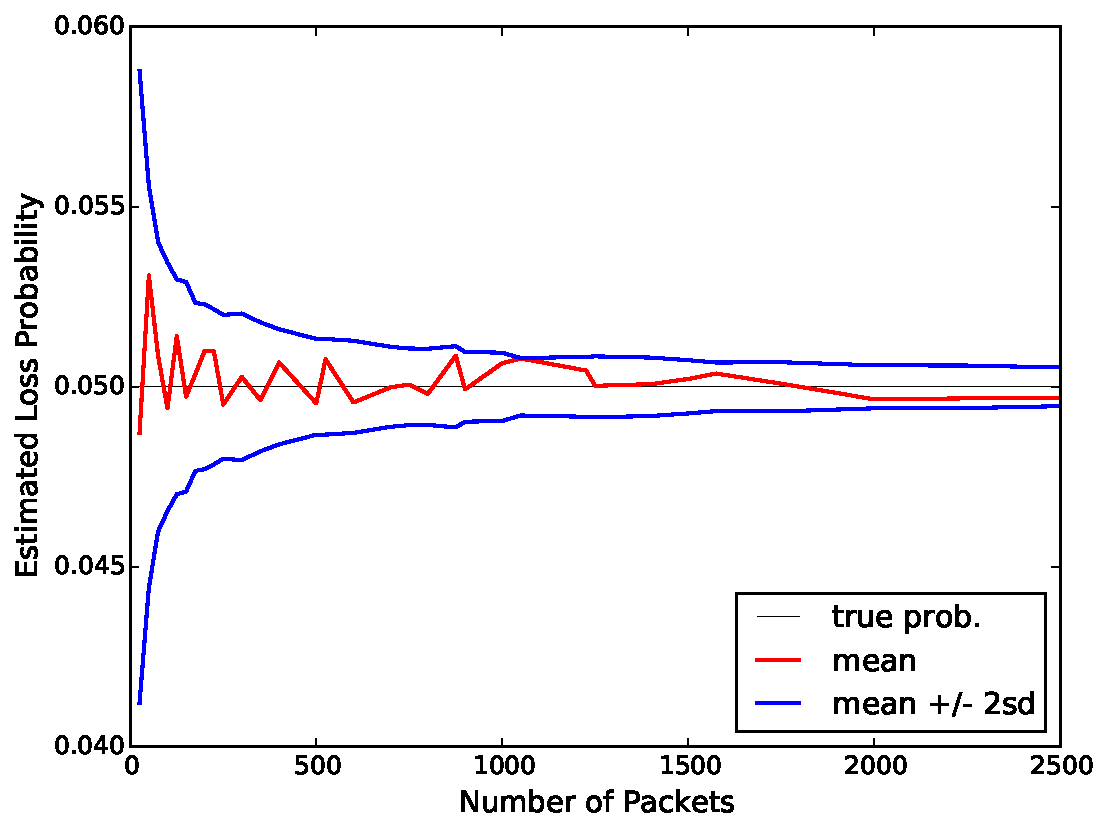
\includegraphics[scale=0.4]{figs/pcount-loss-pkts.pdf}}
    \subfigure[Processing time, with $95\%$ confidence intervals, as a function of number of monitored flows.]{\label{fig:pcount-dtime}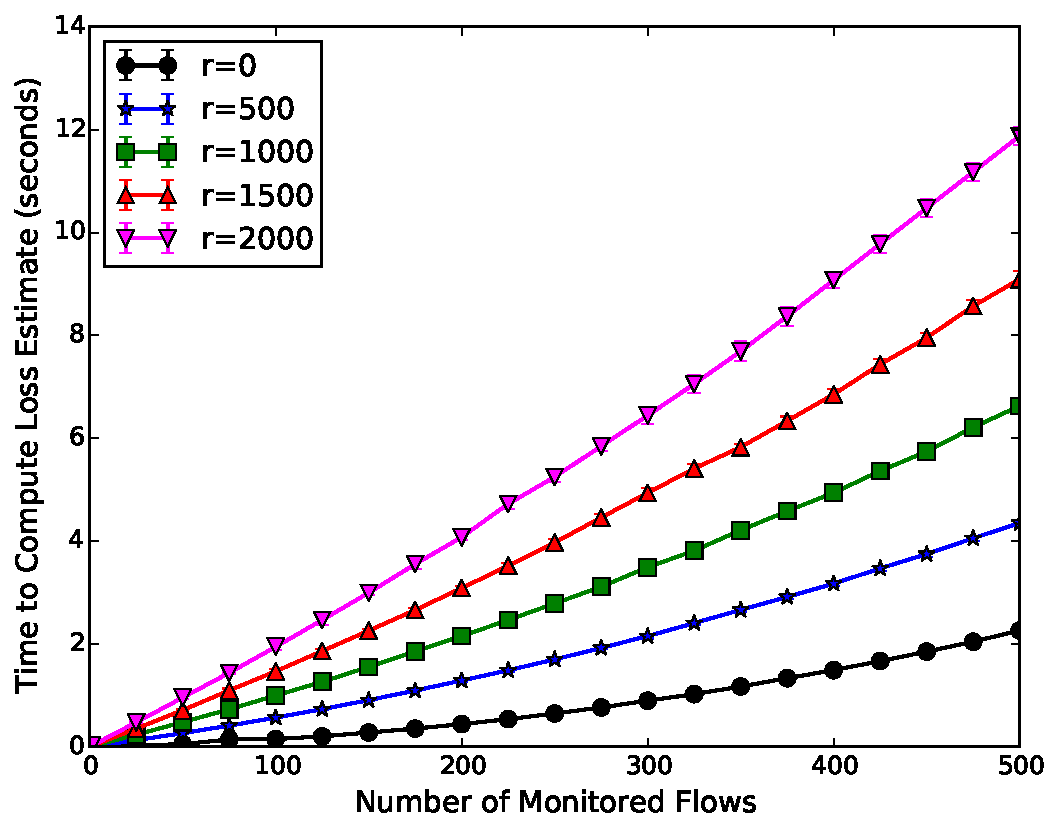
\includegraphics[scale=0.4]{figs/pcount-dtime-w5-j4000.pdf}}
  \end{center}
	\caption{\pcnt results monitoring a single link, $(u,d)$, from Figure \ref{fig:eval-pcount-setup}.}
  \label{fig:pcount-res}
\end{figure*}



\subsection{Backup Tree Installation Simulations}
\label{subsec:eval-backuptrees}

In this section, we simulate the failure of a single link and then measure recovery time, control plane signaling, and garbage collection overhead for \pre and \post both with and without
the \merge optimization. We aim to answer the following questions with these simulations: 
\begin{itemize}
	\item How effective is \steiner in reusing primary tree edges and in providing opportunities for backup tree installation algorithms to reuse primary tree forwarding rules?
	\item How much faster does \pre recover from link failure than \posts? 
	\item How many fewer control messages are needed to install backup trees under \pre versus \posts?
	\item How much control state does \pre pre-install?
	\item In terms of recovery time, control plane signaling, and garbage collection, how much does \merge improve performance relative to \bases?
\end{itemize}
%We use simulations to quantify \pres's faster recovery time relative to \post and \merges's benefits versus \bases: faster recovery time when using \posts, less preinstalled state  under \posts, and reduced garbage collection.  


% Changes to plots: (a)  should label lower bound with algorithm name (e.g., Reactive)

{\bf Setup.}
We use IEEE bus systems $14$, $30$, $57$, and $118$ \footnote{\url{http://www.ee.washington.edu/research/pstca/.}}
and synthetic graphs based on these IEEE bus systems to evaluate our algorithms.  Each bus system consists of buses -- electric substations,
power generation centers, or aggregation points of electrical loads -- and transmission lines connecting those buses. The IEEE bus systems are actual portions of the North American
 transmission network, where PMUs are being deployed.  Note that the bus system number indicates the number of buses (nodes) in the graph (e.g., bus system $57$ has $57$ nodes).  
Synthetic graphs are generated using a procedure described in one of our previous papers \cite{Gyllstrom12} that uses an IEEE bus system as a template to generate
graphs with the same degree distribution as the template bus system.  

We assume that the communication network mirrors the physical bus system topology. It is assumed that
an OpenFlow switch is co-located at each bus and that two unidirectional communication links, one in each direction,
connects these switches following the same configuration as the bus system's transmission lines.  Additionally, we connect each switch with a leaf host using a bidirectional communication link.  
%As a result, each communication network used in our simulations has the same number of hosts and switches.
In this setup, the PMUs measure voltage and current phasors at the buses, then these measurements are sent by the bus's attached host to its first-hop switch, and lastly 
the first-hop switch multicasts the PMU measurements using the network of OpenFlow switches to a set subscribing hosts (terminals).  

For each bus system $n$, we generate synthetic topologies with $n$ switches, $n$ hosts, and set all link weights to $1$.  Then, we randomly create $m=\{1,2,...,\frac{n}{2}\}$ multicast groups, 
each with $n/3$ random terminal hosts, and use the \arbor approximation proposed by Charikar et al. \cite{Charikar98} to compute the $m$ primary trees. \steiners, with $\alpha=1.1$, is then used
to pre-compute, for each primary tree, a backup tree for each primary tree link.
Next, a random communication link, $l$, that is used by at least one primary tree is chosen to fail (i.e., drop enough packets to trigger a \pcnt alert), 
triggering the installation of backup trees using either \post or \pres.  For each $m$, we generate $35$ different synthetic graphs and $3$ random sets of multicast groups, 
yielding a total of $105$ simulation runs per $m$.  
%Primary trees are computed using the \arbor approximation proposed by Charikar et al. \cite{Charikar98} and backup trees computed by \steiner with $\alpha=1.1$. 

The results described in the remainder of this section are those from synthetic topologies generated using IEEE bus system $57$ as a template. The trends are consistent across 
all other networks. Switches in the networks generated using IEEE bus system $57$ have an average diameter of $11.75$ and average degree $3.74$.   
%The $35$ synthetic graphs based on bus system $57$ graphs have an average diameter of $11.75$ and average degree $3.74$. 
For each of the $m$ multicast groups, we initially attempted to multicast packets at a constant rate flow of $60$ packets per second from the root host but this 
caused CPU overload.  Instead, in each simulation run we only initiated the constant rate flows for the primary trees using the failed link.

%{\it Missing the following parameters: link weights are $1$, $\alpha$ for SA computation, what is pcount loss threshold?, how are we inducing loss at links?}


\subsubsection{\steinern Results}
\label{subsubsec:tree-stats}

% assume e2e delay 5ms & 8ms 
The primary trees computed using the \arbor approximation described in Section \ref{subsubsec:steiner-approx} have an average root-to-terminal hop count of $7.54$, while the \steiner backup trees are 
slightly larger with an average end-to-end (E2E) length of $8.4$.  Based on the E2E latency requirements reported in Section \ref{subsec:pmu-requirements}, the 
per-link delay in our simulated topologies would need to be in the range of $0.6-1$ms to satisfy QoS requirements using these multicast trees.  
\footnote{The average root-to-terminal path lengths were largest for IEEE bus system $57$ and the synthetic graphs based on this bus system.  The multicast trees computed for bus system $118$ 
have an average E2E path length approximately $1$ hop fewer than those for bus system $57$, even though IEEE bus system 118 has more than twice as many nodes as bus system $57$.  This is mainly 
due to bus system $118$'s higher density (than bus system $57$). }
%Mainly because bus system $118$ is more dense, its average degree is $4.04$.}
%These latencies are certainly attainable within the portions of the power


%Although IEEE bus system 118 has more than twice as many nodes as bus system $57$, the primary and backup trees computed over bus system $118$ are smaller than those computed
%using bus system $57$.  E2E is a larger graph than  the average E2E path length is  
%This implies that the total per-hop delay must be in the range of $0.6 - 1 $ms to meet the most challenging PMU application E2E latency requirements (Section \ref{subsec:pmu-requirements}).  

On average, the \steiner backup trees have stretch of $1.17$. %, a common goodness measure for multicast trees, of $1.17$.  
Stretch is defined per multicast tree and is the ratio of path length from the root to terminal along the multicast tree to the length of the direct unicast path. 
For comparison with \steiner results, we compute a second backup tree for each primary tree, $T_i^l$, 
by running the \arbor approximation described in Section \ref{subsubsec:steiner-approx} over the original graph with $l$ removed. We denote the set backup trees for $l$ computed using this algorithm
as $B^l$. 
%As expected, the $B^l$ backup trees are smaller than the $\hat{T}^l$ backup trees ($w(\hat{T}^l)/w(B^l) = 1.08$) because $B^l$ trees are computed independent of the primary tree while $\hat{T}^l$

The $B^l$ backup trees are marginally smaller than the $\hat{T}^l$ backup trees: $w(\hat{T}^l)/w(B^l) = 1.08$.  This is expected because $\hat{T}^l$ is computed using 
a heuristic to guide \steiner to reuse primary tree edges, while $B^l$ trees are an approximation of the least cost directed tree (and so are computed independent of the edges used by the primary tree). 

However, $\hat{T}^l$ reuses more primary tree edges ($\hat{T}^l$ reuses $59\%$ of primary tree edges versus $41\%$ under $B^l$). Most importantly, when comparing $\hat{T}^l$ and $B^l$ with 
the primary tree, $\hat{T}^l$ has more common nodes with the primary tree that have the same children in $\hat{T}^l$ and the primary tree ($55\%$ of $\hat{T}^l$ nodes) 
than $B^l$ ($38\%$ of $B^l$ nodes).  
%primary tree and share the same children as its primary tree at $55\%$ of $\hat{T}^l$'s nodes instead of $38\%$ with $B^l$ forwarding rules ($55\%$ instead of $38\%$ with $B^l$).  
This last point is important because this allows $\hat{T}^l$ to reuse more primary tree rules once $\hat{T}^l$ is installed.
In summary, these results suggest that \steiner computes backup trees only slightly larger than an approximation of the least cost tree with a significant gain in primary tree 
edge and forwarding rule reuse. 

%Recall from Section \ref{subsec:steiner} that \steiner first attempts to compute a backup tree, $\hat{T}_i^l$, using a graph copy where 
%the links weights of $\hat{T}_i^l$'s associated primary tree are set to $0$.  If the cost of the resulting backup tree, $\hat{B}_1$, is sufficiently small, $\hat{T}_i^l = \hat{B}_1$ is returned. 
%Otherwise, the minimum cost backup tree, over the original graph without the failed link, is computed and returned.  We denote this second tree as $\hat{B}_2$   In almost all cases $\hat{B}_1$ satisifize
%the cost constraint; on average, $w(\hat{B}_1)/w(\hat{B}_2) = 1.08$.  This modest increase in tree size %link weights of $T_i$

%Graph properties: mean graph diameter=$11.75$, average degree = $3.74$
%Backup Tree properties: avg BT e2E = $8.64$, stretch = $1.17$, $w(BT_1)/w(BT_2) = 1.08$, $c(BT_1)/c(BT_2) = 0.67$, mean percentage PT nodes reused = $78\%$ vs $65\%$, mean percentage PT edges reused = $59\%$ vs $41\%$.

% Graph properties -- degree and diamter (with and without failed link)
% Feasability of E2E latency requirements -- reasonable tree yields PT hop count of x, meaning the avg link delay must be < ?
% Bunchy vs straw man results
% open questions: PT vs BT size, 


%{\bf Signaling Overhead.}
\subsubsection{Signaling Overhead}
\label{subsubsec:eval-signaling}

Next, we compare the number of control messages required to install backup trees as function of the number of primary trees ($m$) installed in the network.  Figure \ref{fig:msgs57} shows the results for 
\post running in \base and \merge mode, referred to as \posts+\base and \posts+\merges, respectively; a lower bound for \post (\posts+\lbs); and \pre in \base mode, denoted as \pres+\bases.  
Note that the results for \pre are the same using \base and \merge because \pre requires 
that only the root node of each backup tree needs to be signaled to activate the backup.  We shall later see how \base and \merge affect the number of forwarding
rules \pre pre-installs.

\posts+\lb computes the lower bound at each switch, $v$, used by a backup tree for the failed link ($l$) and returns the sum of each node's lower bound.
At $v$, the lower bound computation first finds the set of outports used by all primary and backup trees and then eliminates any backup tree with the same outports as a primary tree
(these backup trees can reuse the primary tree forwarding rule rather than installing a new one).  
Among the remaining backup trees, the number of unique sets of outports, $b$, is equal to the minimum number of 
forwarding rules that must be installed at $v$: if fewer than $b$ rules are installed at $v$, packets corresponding to at least one multicast group would not match with a rule that forwards
packets out the correct set of ports.
%Because at least a single flow table entry is needed for each unique set of outports to ensure correct forwarding, the optimal solution cannot be less than the lower bound. 

As expected, we find that \pre requires less signaling overhead than \posts, including even \posts+\lbs.   \pre activates the backup trees by sending a control message
(to install a pre-computed forwarding rule) to the root switch of each of backup tree using the failed link, whereas \post must signal multiple switches to install each 
backup tree. %The mean for $m_l$ starts at $1$ (when $m=1$) and increases linearly as function of $m$ to a maximum of $6.5$ (for $m=28$).  
%(for each backup tree, \post signals each switch with a pre-installed flow under \pres). 

%Likewise, the number of control messages for \bases, \merges, and the lower bound all increase linearly with $m$.  

%{\it TODO: mention that the savings for between $2$ and $2.5$ for $m \geq 15$.}
For \posts, the gap between \base and \merge increases as we introduce more primary trees.  
When $m=1$ there are no opportunities for \merge to consolidate forwarding rules so \merge and \base require exactly 
the same number of control messages to install the backup tree.

As $m$ grows, three factors contribute to an increasing gap between \base and \merges.  One, there are more primary tree forwarding rules 
(installed in the network) that \merge can reuse. Our results show that for $m \geq 7$, $75\%$ of \merge savings (versus \bases) are due to reusing primary tree forwarding rules. Two, 
as $m$ increases more graph edges are used: when $m=28$, $90\%$ of all network links are used by at least one primary tree and is at least $80\%$ for $m \geq10$. 
This benefits \merge because it increases the likelihood that at any switch a backup tree shares the same outgoing links as at least one primary tree. 
%This near network-wide use of graph edges is favorable for \merge because it increases the likelihood that at any switch a backup tree shares the same outgoing links as at least one primary tree. 
Three, as $m$ increases more primary trees are affected by a link failure causing more backup trees to be installed for each link failure. 
This provides additional opportunities for \merge to consolidate flow table entries with other backup trees.
%Three, as $m$ increases more backup trees are installed after a link failure since more primary tree are likely to use $l$. This provides additional opportunities for \merge to consolidate 
%flows with other backup trees. %with common forwarding. 
However, this third factor is less significant than the previous two, as only $25\%$ of \merge savings are due to consolidating flows with other backup trees.
%Overall, the gap between \base and \merge is largest when $m=28$ where \base requires, on average, $271\%$ more control messages than \merges. 

With \posts, \merge does well compared with \lbs. 
On average, \merge requires $25\%$ more control messages than \lbs, suggesting that \merges's local optimization does not miss many opportunities for consolidating flows.
%For all $m \leq 16$, \merge requires at most $25\%$ more control messages than \lb and, in the worst case, is $47\%$ larger than \lbs. 
%These results suggest that \merges's local optimization does not miss many opportunities for consolidating flows.

\subsubsection{Time to Install Backup Trees}
\label{subsubsec:eval-install-time}

%Using the same experimental setup, we estimate the time required to recover from the detected link failure.
%Using our signaling overhead results from the previous section along with measure
Here we compare the time required by each of algorithms to install backup trees.  %Here we estimate the time to install all backup trees. 
Specifically, we measure the time between when the link failure is detected at the controller to when \emph{all} pre-computed backup tree forwarding rules are installed at the network switches.
We refer to this time duration as $t_c$. 
$t_c$  is a function of the controller transmission delay 
(i.e., the time between when the first and last precomputed control messages are sent from the controller), the controller to switch RTT, and the time to install a forwarding rule at a switch.  

We find the transmission delay to be negligible: on average, transmission delay is less than $2.8\%$ and $0.9\%$ of the time to install a \emph{single} flow table entry at a switch,
for \posts+\base and \posts+\merges, respectively.  Even if we conservatively assume that the inter-arrival time of installation messages at each switch is equal to the total transmission delay,
it follows that each switch receives all control messages before completing the installation of its first backup tree rule.  Because rules are installed in parallel across switches, 
the time to install all backup tree rules occurs when the switch with the most backup tree rules to install, $s_x$, installs its last rule.  If we assume $s_x$ has $c_x$ rules to install, let $t_d$ 
be the total transmission delay, and denote the average latency to install a single rule at an OpenFlow switch as $t_i$, then 
     $$t_c = \frac{1}{2}RTT + t_d + c_x(t_i)$$
	 
Because Mininet lacks performance fidelity, we determine $t_i$ values using measurement results from the literature \cite{Ferguson13}, rather than measure rule installation times in Mininet.  
Specifically, we assume the mean installation time per rule is $7.12$ms, as reported by Ferguson et al. \cite{Ferguson13} using the Pronto 3290 OpenFlow switch running the Indigo 2012.09.07 firmware.
%Because Mininet lacks performance fidelity we use flow table entry install times from a real OpenFlow switch (the Pronto 3290 switch running the Indigo 2012.09.07 firmware)
%Unfortunately, because Mininet uses software rather than hardware switches, measuring switch installation times, $t_i$, in Mininet does not yield results that resemble those of 
%real OpenFlow hardware switches.  Instead, we apply flow table entry installation times reported in the literature \cite{Ferguson13} measured using the Pronto 3290 switch running the 
%Indigo 2012.09.07 firmware%to our equation for $t_c$.  Specifically, we assume mean installation time per rule of $7.12$ ms \cite{Ferguson13}.  

Figure \ref{fig:install-time57} shows the estimated elapsed time to install all backup trees as a function of $m$.  We set $RTT=0$ in this simulation.  The trends for each algorithm are a function 
of their $c_x$ values, the maximum number of rules any switch must install,  found at each $m$.  With \pres, $c_x$ is always $1$.  
The difference in total installation time between \posts+\base and \posts+\merge is small in absolute terms (at most $25$ms) because the install times depend on the amount of rule
consolidation each algorithm is able to apply at a single switch, $s_x$, rather than the level of rule sharing possible at multiple switches (as we observed with signaling overhead results).
Nonetheless, the extra milliseconds saved using \merge can be valuable to critical PMU applications.
%While the different installation times between \posts+\bases, \posts+\merges, and \posts+\lb reflect the amount of rule consolidation each algorithm is able to apply at $s_x$. 
%For this reason the difference in total installation time between \posts+\base and \posts+\merge is small in absolute terms (at most $25$ms), 
%however, these extra milliseconds are valuable to critical PMU applications.
%Although the largest difference between \posts+\base and \posts+\merge is small in absolute terms (at most $25ms$), these extra milliseconds are valuable to critical PMU applications.

%{\bf Flow Table Size.}
\subsubsection{Switch Flow Table Size}
\label{subsubsec:eval-table-size}
In our Section \ref{subsubsec:eval-signaling} simulations we found that \pre incurs less signaling overhead than \posts. 
Here we show that these savings come at a cost: \pres's pre-installed forwarding rules can account for a significant portion of limited OpenFlow switch capacity.
%Here we show that these savings come at a cost and quantify this penalty; \pre pre-installs large numbers of forwarding rules at the network switches resulting in  bloated flow tables.

Using the same setup as the other simulations in this section, we record the number of pre-installed backup tree rules at each switch during each simulation run.  
Figure \ref{fig:preinstall57} shows the mean number of pre-installed rules per switch, $r$, as a function of $m$. 
The confidence intervals are omitted because of high variance (during each simulation run, individual counts range from $0$ to $525$.) 
%The confidence intervals are omitted because the number of pre-installed rules has high variance (during each simulation run, individual counts range from $0$ to $525$.) 
\post is not included because it does not pre-install forwarding rules.  The number of pre-installed rules for \pres+\lb is computed using the same algorithm described in Section 
\ref{subsubsec:eval-signaling} for \posts+\lbs. % but applied to all backup trees rather than just $\hat{T}^l$.
%Because \pre installs backup tree forwarding rules only after link failure is detected and garabage collects any stale forwarding rules, \post has the minimum possible aff

Similar to our \post signaling overhead findings, \merge yields up to $2.5$ times better performance than \bases.
\merge and \lb savings increase with $m$ because more primary tree flows are reused and more backup tree rules are shared as $m$ grows.
As a result, the number of pre-installed forwarding rules per backup tree decreases linearly as $m$ increases causing the rate at which $r$ increases for \pres+\merge to slow.

In contrast, $r$ increases linearly with $m$ using \pres+\bases. For each backup tree, \base is only able to avoid pre-installing a forwarding rule at a switch, $v$,
if the backup tree uses the same outports as its primary tree at $v$.  Because this condition depends only on the relationship between a backup tree and its primary tree, the number of
pre-installed rules per backup tree is constant for all $m$.  Since larger $m$ implies more backup trees, $r$ increases linearly with $m$.   
%On the other hand, with \base this value, on average, is constant for all $m$. For each backup tree, \base is only able to avoid preinstalling a forwarding rule at a switch, $v$,
% if the backup tree uses the same outports as its primary tree at $v$.  Because these savings depend only on the relationship between a backup tree and its primary tree, tese savings are
% independent of $m$ becaus % based on overlap between a backup and its primary tree

Based on maximum flow table sizes of real OpenFlow switches (ranging from approximately $1500$ to $1900$ flow table entries \cite{Curtis11,Ferguson13}), at most $r$ occupies  
$19\%$ and $6.7\%$ of flow table space for \pres+\base and \pres+\merges, respectively.  We find that the switch with the most pre-installed forwarding rules (across all simulation runs) 
has at most has $525$ pre-installed forwarding rules (occurs with \pres+\base when $m=28$).  At most, this accounts for $35\%$ of the switch's flow table capacity. %should be $12\%$ capacity for Merger



% MAX: function of number of PT size and number of primary trees ( can show -- graph # vs max # preinstalled for different m
% IEEE 14: PT size = 7,  (m= 5 , max= 25 )           
% IEEE 30: PT size = 14, (m=5, max= 50, 55 ); 	 (m=15 , max=x, 150,175 )
% IEEE 57: PT size = 32, (m=5, max= 100, 110  ); (m=15 , max=, 200, 290, 310);  (m=25 , max=350,450,700)
% IEEE 118: PT size = 68, (m=5 , max=200,210);   (m=15, max= x, 650, 750  )  ;  (m=25 , max=x, 900,1400)

%{\it TOOO discuss max flow table size}.

\subsubsection{Garbage Collection Overhead}
\label{subsubsec:eval-garbage}

After a link $l$ fails, forwarding rules corresponding to primary trees using $l$ may become stale (detailed in Section \ref{subsec:garbage}).
These stale rules are deleted as part of \mdr garbage collection.  In this section, we first we describe garbage collection results for \post and then for \pre using the same simulation
setup described at the start of Section \ref{subsec:eval-backuptrees}.
\posts+\lb and \pres+\lb are both computed based on the \lb algorithm described in Section \ref{subsubsec:eval-signaling}. % and Section \ref{subsubsec:eval-table-size}, respectively.
%The lower bound for \post and \pre, \lbs, is based on the same algorithm 
%when a backup tree is installed in response to a link failure, $l$, forwarding rules corresponding to primary trees using $l$ 
%may become unused.  These stale rules are deleted as part of our garbage collection procedure.  % we first describe our results using \
%More precisely, consider a primary tree using $l$, $T^l_i$.  Each of $T^l_i$'s forwarding rules belongs to one of the following three categories: 
%(1) the rule is reused by backup tree for $l$ ($\hat{T}^l_i$), (2) the rule is reused by another primary tree's backup tree (e.g., $\hat{T}^l_j$ where $i\neq j$) and
%(3) the rule is not reused by any backup tree for $l$ or other primary tree.  Category (3) rules become stale when $l$ fails and are garbage collected. 

{\bf \post Garbage Collection.}
%Primary tree flow rules become stale when one of its links fail and the rule is not used by its backup tree nor any other tree installed in the network.  
Figure \ref{fig:reactive-garbage57} shows a modest delta in the number of stale rules between \bases, \merges, and \lbs. For each of these algorithms, on average $55\%$ of primary
tree rules are reused by its backup tree (and are therefore not garbage collected).
\footnote{Because all three algorithms use \steiner to compute backup trees this statistic is the same for \posts+\bases, \posts+\merges, and \posts+\lbs.}
This implies that \posts+\merge and \posts+\lb are only able to reduce garbage collection over the remaining  $45\%$ of primary tree rules. 
Among these remaining primary tree rules, \posts+\merge and \posts+\lb reduce garbage collection when any backup tree for $l$ reuses a primary tree rule.  Our results
show that this yields small savings in garbage collection.
%Among the remaining $45\%$ of primary tree rules, \posts+\merge and \posts+\lb reduce garbage collection relative to \posts+\base when any backup tree for $l$ reuses a primary tree rule.  

%Approximately $45\%$ of primary tree rules created using \base are garbage collected, the other $55\%$ of rules belong to category (1) as only \merge rules can be in category (2).  For each $m$, 
%the number of stale \base rules is nearly identical to the number of control messages required by \base (at most $2\%$ fewer stale rules than \base control messages).  This similarity is due to
%backup trees being nearly identical in size as their corresponding primary tree: on average each backup tree has $1.5\%$ more nodes than its primary tree.  

%Among the remaining $45\%$ of primary tree rules, \posts+\merge and \posts+\lb reduce garbage collection relative to \posts+\base when 

{\bf \pre Garbage Collection.}
% revised verion: (1) many more backup trees, (2) Basic flow is non-stale if one of its own backup tree reuses, (3) Merger: any of the backup trees.
Compared with \posts, we find a significant decrease in stale flows with \pre because \pre installs up to two orders of magnitude more backup trees, providing
more opportunities for primary tree forwarding rules to be reused.  Recall that \post only installs the backup trees for $l$, whereas \pre pre-installs, for each primary tree, a backup tree for
each primary tree link, amounting to approximately $32$ backup trees per primary tree.  As a result, we observe $2.5$ times fewer stale rules with \pres+\base versus \posts+\base and 
\pres+\merge has up to an order of magnitude decrease in garbage collection versus \posts+\merges.

The number of stale \pres+\merge forwarding rules actually decreases as $m$ grows.  
Recall that for a primary tree using $l$, any of its rules is not stale if at least one other primary or backup tree uses this flow table entry. 
Because the number of pre-installed backup trees is so large (approximately $32m$), for large $m$, nearly all primary tree rules are still used after a link failure (resulting
in a decrease in stale flow table entries as $m$ grows).

%With \pres+\bases, a forwarding rule for primary tree, $T^l_i$, becomes stale (after $l$ fails) only if none of its approximately $32$ backup trees reuse this forwarding rule. In contrast, the same
%forwarding rule is stale under \posts+\base if $T^l_i$'s backup tree for $l$ does not reuse the rule.   Since over thirty times more backup trees per primary tree are candidates to reuse
%a primary tree rule with \pre versus \posts, we observe $2.5$ times fewer stale rules with \pres+\base.

%\merge has the largest decrease in garbage collection with \pre versus \posts. With \posts+\merges, a primary tree ($T^l_i$) rule can be reused by $T^l_i$'s backup tree for $l$ ($\hat{T}^l_i$) or 
%by another primary tree's backup tree for $l$ (e.g., $\hat{T}^l_j$ where $i\neq j$).  By contrast, $T^l_i$'s primary tree flows can be reused by any of the approximately $32m$ backup trees 
%pre-installed in the network. As a result, up to an order of magnitude (when $m=28$) fewer stale flows are found with \pres+\merge and the number of stale \merge forwarding rules actually decreases
%as $m$ grows.  

\subsubsection{Summary}

In summary, we found that as more primary trees are installed in the network, the gap between \merge and \base grows (for both \post and \pres) in terms of signaling overhead, 
total backup tree installation time, number of pre-installed forwarding rules, and garbage collection overhead.  The is the case 
because, with larger $m$, there are more opportunities for \merge to reuse primary tree rules and consolidate rules among other backup trees.

Additionally, we found \pre yields fewer control messages and faster recovery than \post -- \post sends up to $10$ times more control messages than \pre --
but at the cost of storage overhead at each switch. \pres's pre-installed backup trees can account for as much as $35\%$ of the capacity reserved for wild-card matching rules 
of a conventional OpenFlow switches \cite{Curtis11}. However, when applying \merge to \pres, this statistic drops to $20\%$ and, on average, \pres+\merge accounts for only $6.7\%$ of flow
table capacity.
%should be $12\%$ capacity for Merger


%Our findings for \pres+\merge suggests that the system of multicast trees installed using \merge rule instantiation become stable -- in terms of rules that must be installed for each additional 
%multicast tree and garbage collection overhead -- as more primary trees are supported.  In section \ref{subsubsec:eval-table-size}, we found that the mean number of pre-installed forwarding rules 
%levels off as $m$ increases, suggesting that fewer new rules must be installed for each additional multicast tree.  Also, garbage collection actually decreases as more $m$ grows (Section
%\ref{subsubsec:eval-garbage}).

%The inverse relationship between stale rules and $m$ suggests that the system of multicast trees installed using \merge rule instantiation become stable -- minimal garbage collection
%is needed after a link fails and few new rules when more primary trees are supported. 






%As a result, with \pres the forwarding rule of each primary tree using $l$ is not stale if any of its $|\hat{E}|$ backup trees reuse the rule. 
%However, with \post it must be the case the single backup tree for $l$ must reuse a primary tree rule.  For this reason, we observe, on average, $2.5$ times fewer \base stale rules with \pres. 



%Garbage collection: 
%	- for \bases, first we consider the set of garbage nodes for the failed link.  Then, all of the primary tree's backup trees are examined to determine if any uses the garbage node.
%	- \merge primary tree flows can be reused by any backup tree, rather than just primary tree's own backups, thereby reducing the number of stale flows 



%Furthermore, each backup tree -- with \bases, \merge -- reuses approximately $55\%$ of its corresponding primary tree's forwarding rules, further reducing the  	


%are both more primary trees installed in the network with forwarding rules that \merge can reuse
%and more candidate backup tree flow table entries that can be consolidated using \merges.  Thus, 
% larger m ==> more primary tree flows to reuse.  good covereage, 90% of graph edges are used by at least one PT.  
% larger m ==> more backup trees

%The ratio starts at $1$ when $m=1$ and increasing to a maximum of $2.71$ when $m=28$. As more $m$ grows, on average there are both more backup tree flow table entries that can be consolidate using
%\merge and more primary trees installed in the network that \merge can reuse, and thereby save additional sending more control messages.


%MISSING:
%		* what percentage of same PT nodes are resused --> comment on SA algorithm
%		* what is the node+edge coverage of primary trees. 
%				- what percentage of savings are based on are from PT reuse, BT reuse   (SEE Garbage results for these stats)
%
	


%We compare the recovery time -- measured as the time from when the link failure was detected to when all $\hat{T}^l$ flows entries are installed -- 
%as function of the amount of overlap between the primary and backup tree (measured by $B^l$ and defined in Section \ref{subsec:install-backups} as the number of forwarding rules unique to $\hat{T}^l$).



\begin{figure*}[t]
  \begin{center}
    \subfigure[Number of control messages to activate backup trees.]{\label{fig:msgs57}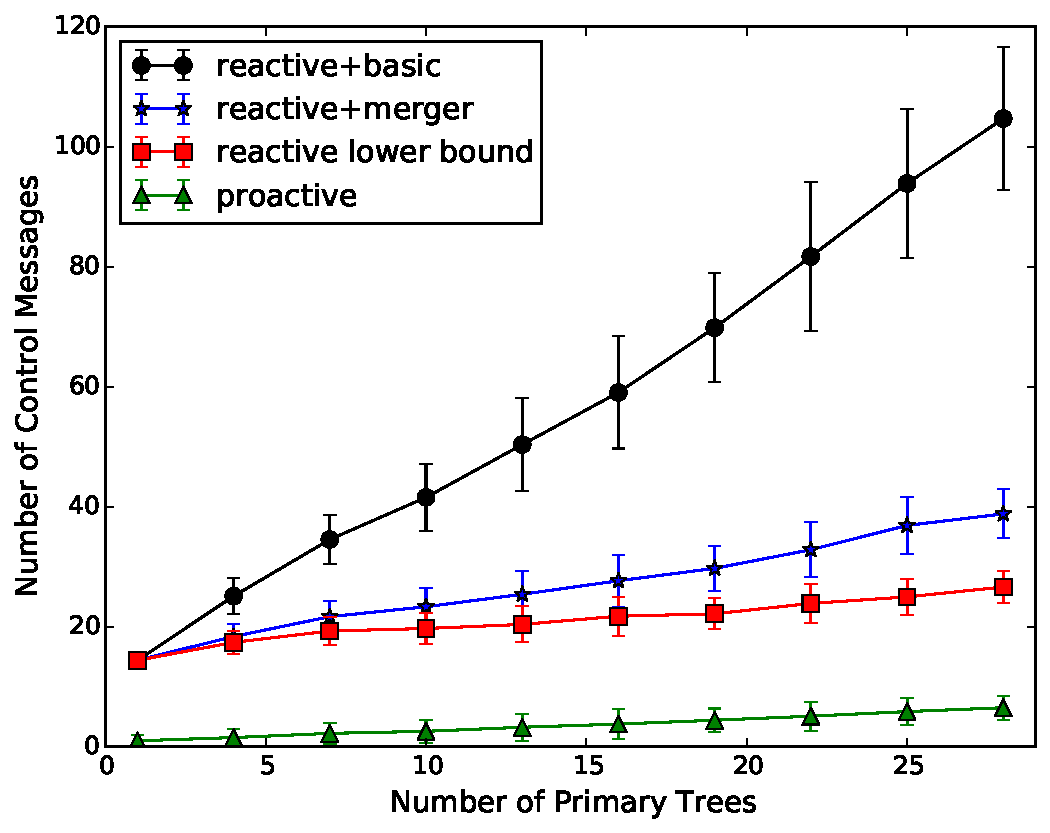
\includegraphics[scale=0.4]{figs/msgs-ieee57.pdf}}
	\subfigure[Total time to install all backup tree flow table entries.]{\label{fig:install-time57}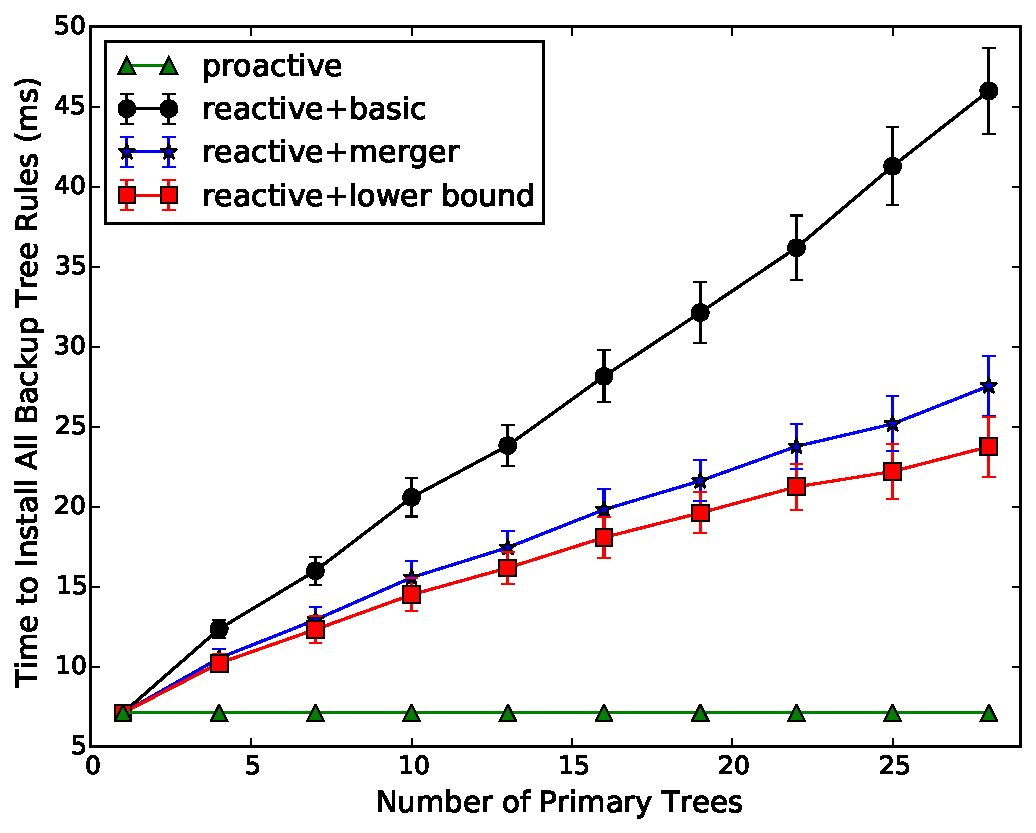
\includegraphics[scale=0.4]{figs/install-time-ieee57.pdf}}
	\subfigure[\pres: mean number of pre-installed rules per switch.]{\label{fig:preinstall57}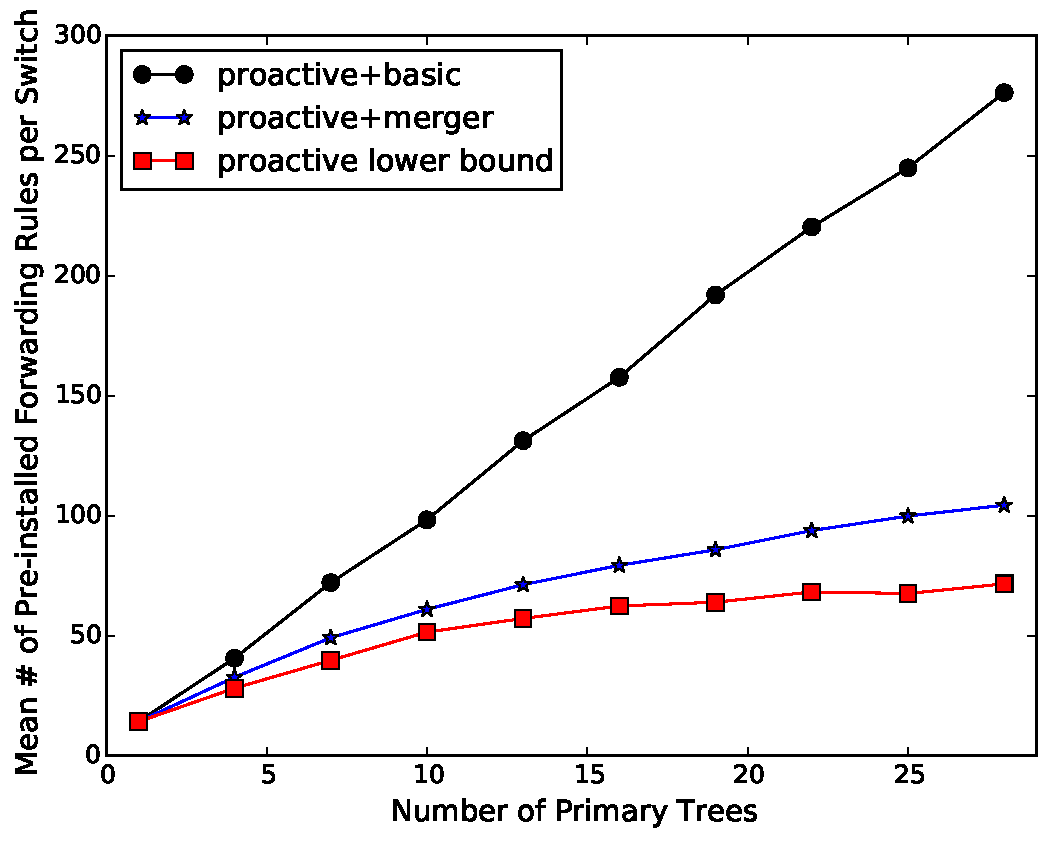
\includegraphics[scale=0.4]{figs/preinstall-ieee57.pdf}}
    %\subfigure[\pres: maximum number of pre-installed rules at a single switch]{\label{fig:preinstall-max57}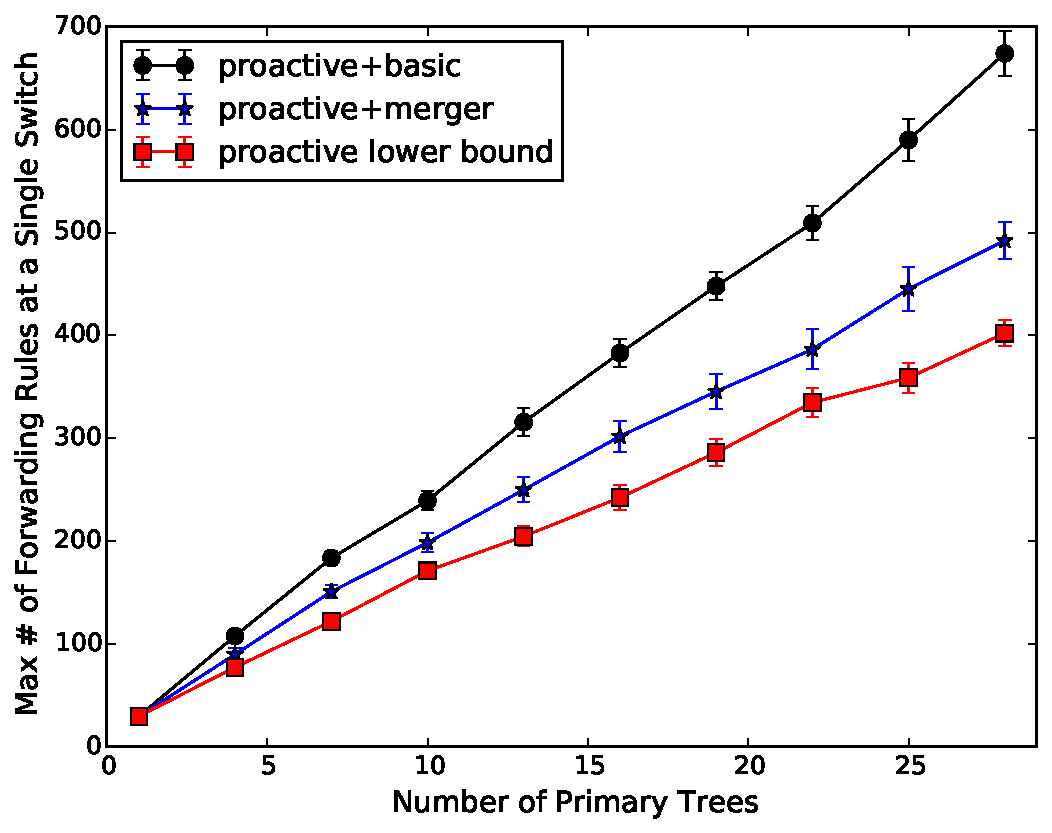
\includegraphics[scale=0.31]{figs/preinstall-max-ieee57.pdf}}
	\subfigure[\posts: number of stale flow table entries resulting from link failure. ]{\label{fig:reactive-garbage57}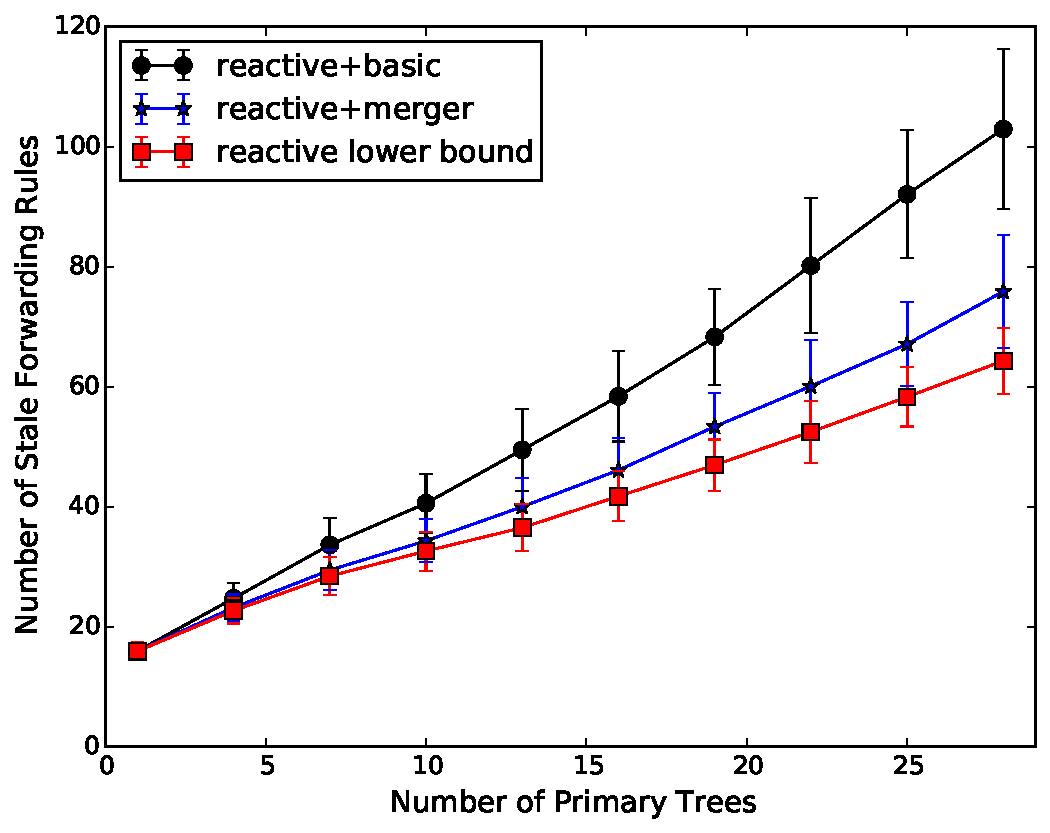
\includegraphics[scale=0.4]{figs/garbage-ieee57.pdf}}
    \subfigure[\pres: number of stale flow table entries resulting from link failure. ]{\label{fig:preinstall-garbage57}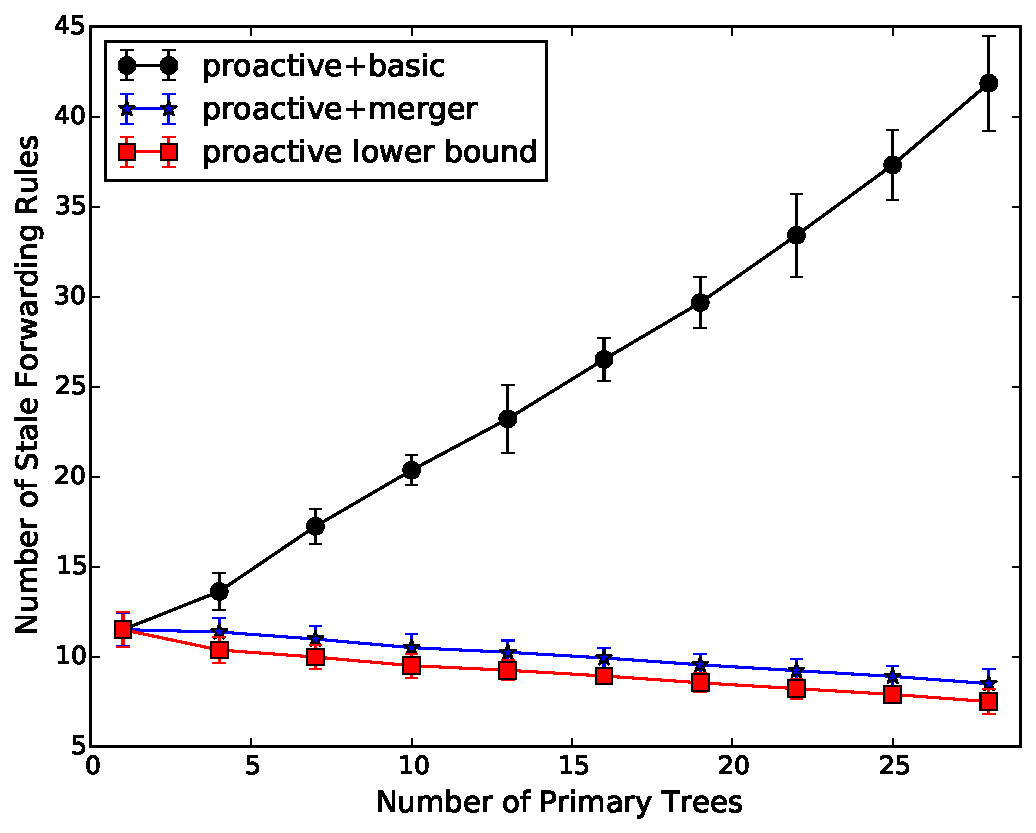
\includegraphics[scale=0.4]{figs/preinstall-garbage-ieee57.pdf}}
  \end{center} 
	\caption{\post and \pre results for a single random link failure of synthetic topologies based on IEEE bus system $57$. 
	Each data point is the mean over $105$ simulation runs and the $95\%$ confidence interval is shown in all plots expect (c).} %\ref{fig:preinstall57}.}
  \label{fig:msgs-preinstall57}
\end{figure*}




\section{Conclusions}
\label{sec:conclude}

We addressed reliable multicasting of critical Smart Grid data.
%In summary, we addressed the problem of providing reliable multicast data dissemination of critical Smart Grid data. 
Towards this goal, we designed, implemented, and evaluated a suite of algorithms that collectively provide fast packet loss detection and fast rerouting using pre-computed backup multicast trees. 
Because this required making changes to network switches, we used OpenFlow to modify switch forwarding tables to execute these algorithms in the data plane.
%according to the rules generated at Using SDN abstractions

%First, we presented \pcnts, an algorithm that uses OpenFlow primitives to tag and count individual packets, allowing for accurate packet loss detection of individual links at small time scales.
First, we presented \pcnts, an algorithm that used OpenFlow primitives to accurately detect per-link packet loss inside the network rather than using slower E2E measurements. % at small time scales.
%OpenFlow packet counters and ability to mark individula packets to provide  accurate packet loss detection at small time scales. 
Next, we formulated a new problem, \mcs, that considered computing
backup trees that reuse edges of already installed multicast trees as a means to reduce control plane signaling.  \mc was proved to be at least NP-hard
so we designed an approximation algorithm called \steiners.  Lastly, we presented two algorithms, \pre and \posts, that installed backup trees at OpenFlow controlled switches. 
As an optimization to \pre and \posts, 
we introduced \merges, an algorithm that consolidated forwarding rules at switches where multiple trees had common children.
%we introduced \merges, an algorithm built on the observation that forwarding rules can be consolidated at switches where multicast trees have common children.  
%When applied to \pres, \merge reduce the amount of pre-installed control state and with \post results in fewer control messages. 


Mininet simulations were used to evaluate our algorithms over communication networks that mirrored the structure of IEEE bus systems (actual portions of the North American power grid).
We found \pcnt estimates were accurate when monitoring even a small number of flows over short time window: after sampling only $75$ packets, the $95\%$ confidence interval of \pcnt loss estimates 
were within $15\%$ of the true loss probability. By pre-installing 
backup trees, \pre resulted in up to a ten-fold decrease in control messages compared with \posts, which had to signal multiple switches to install each backup tree. 
However, in scenarios with many multicast groups, \pres's pre-installed forwarding rules accounted for a significant portion of scarce OpenFlow switch table capacity (up to $35\%$ of
a standard OpenFlow switch). Fortunately, \merge reduced the amount of pre-installed forwarding state by a factor of $2-2.5$, to acceptable levels.


% MOVED THIS TO THESIS CONCLUSION CHAPTER
%As future work, several problems remain unaddressed. One problem of interest is using optimization criteria different from \mcs's objective function to compute backup trees and then evaluate
%\pres, \posts, and \merge performance using these backup trees.  For example, backup trees may be computed with the goal of protecting against the worst-case impact of a subsequent link failure
%by minimizing the maximum number of multicast trees using a single link
%It is unknown how effective our installation algorithms would be given these types of backup trees.
%Measurements using real OpenFlow hardware switches would strengthen our \pcnt processing time and backup tree installation time results, which both suffered from inaccuracies due to Mininet's
%performance fidelity issues.  
%Lastly, the problem \merge addresses -- find the minimum number of forwarding rules for a set of multicast trees -- has unknown complexity.
%We conjectured that this problem is NP-hard in Section \ref{subsubsec:merge-discuss}.



%}



%%
%% Beginning of back matter
\backmatter  %% <--- mandatory

%%
%% We don't support endnotes

%%
%% A bibliography is required.
\bibliographystyle{umthesis}
\bibliography{chapter3}
\end{document}

%%% Local Variables: 
%%% mode: latex
%%% TeX-master: t
%%% End: 
